\begin{abox}
	Net-December-2019
	\end{abox}
\section{PART A}
\begin{enumerate}
	\item A two-digit number is such that if the digit 4 is placed to its right, its value would increase by 490 . Find the original number.
	 \begin{tasks}(4)
		\task[\textbf{a.}]48
		\task[\textbf{b.}]54
		\task[\textbf{c.}]64
		\task[\textbf{d.}] 56
	\end{tasks}
\begin{answer}
	\begin{align*}
	\text{ Let the two digit}&\text{ number be $10 x+y$}\\
\text{	From the question}&\\
	100 x+10 y+4-(10 x+y)&=490 \Rightarrow 90 x+9 y=486 \Rightarrow 9(10 x+y)=486\\
\text{	Therefore, }10 x+y&=\frac{486}{9}=54
	\end{align*}
			So the correct answer is \textbf{Option (b)}
\end{answer}
\item  Given that $K !=1 \times 2 \times 3 \times \ldots \times K$, which is the largest among the following numbers?
	 \begin{tasks}(4)
		\task[\textbf{a.}]$(2 !)^{1 / 2}$
		\task[\textbf{b.}]$(3 !)^{1 / 3}$
		\task[\textbf{c.}] $(4 !)^{1 / 4}$
		\task[\textbf{d.}] $\frac{(3 !)}{2}$
	\end{tasks}
\begin{answer}
	\begin{align*}
(2 !)^{1 / 2}&=\left(2^{6}\right)^{1 / 12}=(64)^{1 / 12},(3 !)^{1 / 2}=\left(6^{4}\right)^{1 / 12}=(1296)^{1 / 12}\\
	(4 !)^{1 / 4}&=\left(24^{3}\right)^{1 / 12}=(13824)^{1 / 12}, \frac{(3 !)}{2}=3=\left(3^{12}\right)^{1 / 12}=(43046721)^{1 / 12}\\
\text{	Hence }&\frac{(3 !)}{2}\text{ is largest}
	\end{align*}
		So the correct answer is \textbf{Option (d}
\end{answer}
\item  Of three children, Uma plays all three of cricket, football and hockey. Iqbal plays cricket but not football and Tarun plays hockey but neither football nor cricket. The number of games played by at least two of the children is
	 \begin{tasks}(4)
		\task[\textbf{a.}] One
		\task[\textbf{b.}]Two
		\task[\textbf{c.}]Three
		\task[\textbf{d.}]  zero
	\end{tasks}
\begin{answer}
 From the table we see that cricket is played by two children and Hockey is also played by two children. Football is played by just one student.\\\\
 \renewcommand*{\arraystretch}{1.5}
 \begin{tabular}{|l|c|c|c|}
 	\hline & Cricket & Football & Hockey \\
 	\hline Uma & $\checkmark$ & $\checkmark$ & $\checkmark$ \\
 	\hline Iqbal & $\checkmark$ & $\mathrm{X}$ & \\
 	\hline Tarun & $\mathrm{X}$ & $\mathrm{X}$ & $\checkmark$ \\
 	\hline
 \end{tabular}\\\\
Hence number of games played by at least two of the children $=2$\\
	So the correct answer is \textbf{Option (b}
\end{answer}
\item  A multiple choice exam has 4 questions, each with 4 answer choices. Every question has only one correct answer. The probability of getting all answers correct by independent random guesses for each one is
	 \begin{tasks}(4)
		\task[\textbf{a.}]14
		\task[\textbf{b.}]$(1 / 4)^{4}$
		\task[\textbf{c.}] $(3 / 4)$
		\task[\textbf{d.}] $(3 / 4)^{4}$
	\end{tasks}
\begin{answer}
	\begin{align*}
	\renewcommand*{\arraystretch}{1.5}
	&\begin{array}{|c|c|c|c|}
	\hline \text { First question } & \text { Second question } & \text { Third question } & \text { Fourth question } \\
	\hline 4 \text { ways } & 4 \text { ways } & 4 \text { ways } & 4 \text { ways } \\
	\hline
	\end{array}
	\end{align*}
	\begin{align*}
\text{	Each question can be answered}&\text{ in 4 ways. Hence total number of ways of answering the} \\
\text{four questions }&=4 \times 4 \times 4 \times 4=4^{4}\\
\text{	There is only one }&\text{way of providing the correct answer}\\
\text{	Hence, required probability }&=1 / 4^{4}
	\end{align*}
		So the correct answer is \textbf{Option (b}
\end{answer}
\item  The result of a survey to find the most preferred leader among $A, B, C$ is shown in the table\\\\
\renewcommand*{\arraystretch}{1.5}
	\begin{tabular}{|c|c|c|c|}
		\hline Votes & $A$ & $B$ & $C$ \\
		\hline $1^{\text {st }}$ preference & 13 & 54 & 33 \\
		\hline $2^{\text {nd }}$ preference & 24 & 37 & 39 \\
		\hline $3^{\text {rd }}$ preference & 63 & 9 & 28 \\
		\hline
	\end{tabular}\\\\
 First, second and third preferences are given weights $3,2,1$, respectively. Statistically, which of the following can be said to represent the preferences of the voters?
	 \begin{tasks}(1)
		\task[\textbf{a.}]$A$ and $C$ are within $10 \%$ of each other
		\task[\textbf{b.}]$B$ is the most preferred
		\task[\textbf{c.}]$B$ and $C$ are within $10 \%$ of each other
		\task[\textbf{d.}] $C$ is the most preferred
	\end{tasks}
\begin{answer}
	\begin{align*}
	\text{ Taking into account }&\text{their respective weights}\\
	\text{Number of votes of }A&=13 \times 3+24 \times 2+63 \times 1=150\\
	\text{Number of votes of }B&=54+37 \times 2+9 \times 1=245\\
\text{	Number of votes of }C&=33 \times 3+39 \times 2+28 \times 1=205\\
	\text{Hence we can say that }&\text{$B$ is most preferred.}
	\end{align*}
		So the correct answer is \textbf{Option (b}
\end{answer}
\item  Which is the curve in the figure whose points satisfy the equation $y=\operatorname{constant} \times e^{x} ?$
	 \begin{tasks}(4)
		\task[\textbf{a.}]A
		\task[\textbf{b.}]B
		\task[\textbf{c.}]C
		\task[\textbf{d.}] D
	\end{tasks}
\begin{figure}[H]
	\centering
	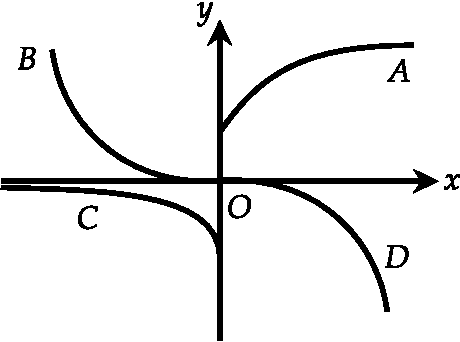
\includegraphics[height=3cm,width=4cm]{Net-D-19-1}
\end{figure}
\begin{answer}
	\begin{align*}
	 \text{The graph of the curve }y&=k \times e^{x}\text{ is shown in the figure for}\\
	k>0 \text { and }& k<0 \text {. }\\
	\text{Hence the correct}&\text{ option is (c)}
	\end{align*}
	\begin{figure}[H]
		\centering
		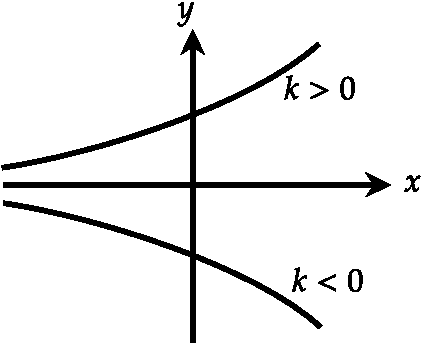
\includegraphics[height=3cm,width=4cm]{Net-D-19-2}
	\end{figure}
	So the correct answer is \textbf{Option (c)}
\end{answer}
\item An ice cube of volume $10 \mathrm{~cm}^{3}$ is floating over a glass of water of $10 \mathrm{~cm}^{2}$ cross-section area and $10 \mathrm{~cm}$ height. The level of the water is exactly at the brim of the glass. Given that the density of ice is $10 \%$ less than that of water, what will be the situation when ice melts completely?
 \begin{tasks}(1)
	\task[\textbf{a.}] The level falls by $10 \%$ of the side of the cube.
	\task[\textbf{b.}] The level falls by $10 \%$ of the original height of the water column
	\task[\textbf{c.}]The level increases by $10 \%$ of the side of the cube and water spills out
	\task[\textbf{d.}]  There is no change in the level of the water.
\end{tasks}
\begin{answer}
	\begin{align*}
	\text { Let the density of water be }& \rho \omega \text { then density of ice }=\frac{9 \rho \omega}{10}\\
	\text{For floating}\\
	\text{Weight of cube }&=\text{ Buoyant force}\\
	\Rightarrow \rho_{i} v_{i} g&=\rho_{\omega} v g \Rightarrow \frac{9 \rho \omega}{10}\left(10 \mathrm{~cm}^{3}\right)=\rho_{\omega} v \Rightarrow v=9 \mathrm{~cm}^{3}
	\intertext{hence $9 \mathrm{~cm}^{3}$ if ice is initially sulomerged in water when ice melts its volume changes from $10 \mathrm{~cm}^{3}$ to $\left(10 \mathrm{~cm}^{3}\right) \times \frac{9}{10}=9 \mathrm{~cm}^{3}$. Thus we see that there is no change in the level of water.}
	\end{align*}
		So the correct answer is \textbf{Option (d)}
\end{answer}
\item  In a college admission where applicants have to choose only one subject, $1 / 4^{\text {th }}$ of the applicants opted for Biology. $1 / 6^{\text {th }}$ for chemistry, $1 / 8^{\text {th }}$ for Physics and $1 / 12^{\text {th }}$ for Maths. 18 applicants did not opt for any of the above four subjects. How many applicants were there?	
 \begin{tasks}(4)
	\task[\textbf{a.}]22
	\task[\textbf{b.}]24
	\task[\textbf{c.}]36
	\task[\textbf{d.}] 48
\end{tasks}	
\begin{answer}
	\begin{align*}
	\text{Let here be $x$ applicants}\\
\text{	From the question}\\
	x-\left(\frac{x}{4}+\frac{x}{6}+\frac{x}{8}+\frac{x}{12}\right)=18 \Rightarrow x-\frac{15 x}{24}&=18 \Rightarrow \frac{9 x}{24}=18 \Rightarrow x=48
	\end{align*}
	So the correct answer is \textbf{Option (d)}
\end{answer}
\item  Based on the bar chart shown here, which of the following inferences is correct?
 \begin{tasks}(1)
	\task[\textbf{a.}]Region $A$ uses maximum water per kg of rice
	\task[\textbf{b.}] Average water consumption of the four regions is
	$37.5$ lakh liters
	\task[\textbf{c.}] Region $D$ uses thrice the amount of water used by region $A$ per $\mathrm{kg}$ of rice.
	\task[\textbf{d.}]  Region $B$ uses 20 lakh litres of less water than region $A$
\end{tasks}	
\begin{figure}[H]
	\centering
	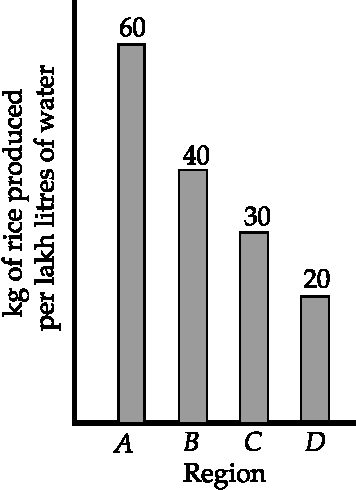
\includegraphics[height=5cm,width=3.5cm]{Net-D-19-3}
\end{figure}
\begin{answer}
	\begin{align*}
	 \text{Water used for the production of rice per }&\mathrm{kg} in \text{four regions $A, B, C$ and $D$ are} \\
	 \frac{1}{60}, \frac{1}{40}, \frac{1}{30}&\text{ and }\frac{1}{20}\text{ respectively}\\
	\text{Since }\frac{1}{20}&=3 \times \frac{1}{60},\text{ hence correct option is (c)}
	\end{align*}
		So the correct answer is \textbf{Option (c)}
\end{answer}
\item  In a race five drivers were in the following situation. $M$ was following $V, R$ was just ahead of $T$ and $K$ was the only one between $T$ and $V$. Who was in the second place at that instant?
	 \begin{tasks}(4)
		\task[\textbf{a.}]$V$
		\task[\textbf{b.}]$R$
		\task[\textbf{c.}]$T$
		\task[\textbf{d.}]$K$ 
	\end{tasks}
\begin{answer}
	\begin{align*}
	\text { From the statement ' } &R \text { was just ahead of } T \text { ', we have the following situation: }\\
	R,T\\
	\text { From the statement ' } &K \text { was the only one between } T \text { and } V \text { we ca write }\\
	R,T,K,V\\
	\text { From the statement ' } &M \text { was following } R \text { ' we can write }\\
	R,T,K,V,M\\
	\text { Hence } &T \text { was in the second place. }
	\end{align*}
	So the correct answer is \textbf{Option (c)}
\end{answer}
\item  A bag contains 8 red balls, 17 green balls. What is the minimum number of balls that needs to be taken out from the bag to ensure getting at least one ball of each colour?
	 \begin{tasks}(4)
		\task[\textbf{a.}]19
		\task[\textbf{b.}]18
		\task[\textbf{c.}]28
		\task[\textbf{d.}] 27
	\end{tasks}
\begin{answer}
Solution: If we draw a red ball then certainly we have drawn at least one ball of each colour.\\
Hence the minimum number of balls that must be drawn to ensure that at least one ball of each colour is drawn $=17+10+1=28$.\\
		So the correct answer is \textbf{Option (c)}
\end{answer}
\item  In a very old, stable forest, a particular species of plants grows to a maximum height of $3 \mathrm{~m}$. In a large survey, it is found that $30 \%$ of the plants have heights less than $1 \mathrm{~m}$ and $50 \%$ have heights more than $2 \mathrm{~m}$. From these observations we can say that the height of the plants increases
	 \begin{tasks}(1)
		\task[\textbf{a.}] At the slowest rate when they are less than $1 \mathrm{~m}$ tall
		\task[\textbf{b.}]At the fastest rate when they are between $1 m$ and $2 m$ tall
		\task[\textbf{c.}]At the fastest rate when they are more than $2 m$ tall
		\task[\textbf{d.}]  At the same rate at all stages
	\end{tasks}
\begin{answer}
From the question we see that $20+50=70$ percent plants have heights more than\\
\begin{figure}[H]
	\centering
	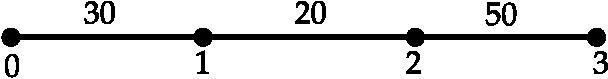
\includegraphics[height=0.7cm,width=5.8cm]{Net-D-19-4}
\end{figure}
in which only $50 \%$ plants have height more than $2 \mathrm{~m}$. Hence plants show maximum rate of increase of height when they are between $1 \mathrm{~m}$ and $2 \mathrm{~m}$.\\
		So the correct answer is \textbf{Option (b)}
\end{answer}
\item  What day of the week will it be 61 days from a Friday?
	 \begin{tasks}(4)
		\task[\textbf{a.}]Saturday
		\task[\textbf{b.}]Sunday
		\task[\textbf{c.}]Friday
		\task[\textbf{d.}] Wednesday
	\end{tasks}
\begin{answer}
	\begin{align*}
\text{ After a given day every $7^{\text {th }}$ day is the same day.}\\
	\text{Now, in 61 days $7 \times 8=56$ th day will be a Friday.}&\text{ Hence 61 th day will be a Wednesday}
	\end{align*}
	So the correct answer is \textbf{Option (d)}
\end{answer}
\item  Which of the following 7 -digit numbers CANNOT be perfect squares?
	$$
	A=45 x y z 26, B=2 x y z 175, C=x y z 3310
	$$
	 \begin{tasks}(4)
		\task[\textbf{a.}] Only A
		\task[\textbf{b.}]Only $B$
		\task[\textbf{c.}]Only $C$
		\task[\textbf{d.}] All three
	\end{tasks}
\begin{answer}
	\begin{align*}
	\text{Only a four digit number when squared can give a }&\text{7 -digit number.}\\
\text{	Suppose }A&=45 x y z 26=(a b c 6)^{2}\\
	\text{But the second digits of }(a b c 6)^{2}&\text{ is always 1 or 3 or 5 or 7}\\
	\text{Suppose }B&=2 x y z 175=(x y z 5)^{2}\\
\text{	But the second last digit of }&(x y z 5)^{2}\text{ is always 2}\\
\text{Suppose }C&=x y z 3310=(p q r 0)^{2}\\
\text{But the second last digit of }&(p q r 0)^{2}\text{ is always 0}
\intertext{Since all three numbers $A, B$ and $C$ do not satisfy the requirements for a perfect square, none of them is a perfect square. Hence the correct option is (d)}
	\end{align*}
	So the correct answer is \textbf{Option (d)}
\end{answer}
\item  A cyclist covers a certain distance at a constant speed. If a jogger covers half the distance in double the time as the cyclist, the ratio of the speed of the jogger to that of the cyclist is
 \begin{tasks}(4)
	\task[\textbf{a.}] $1: 4$
	\task[\textbf{b.}]4:1
	\task[\textbf{c.}] $1: 2$
	\task[\textbf{d.}] 2:1
\end{tasks}
\begin{answer}
	\begin{align*}
	\text{ Let the speed of cyclist be $v$ and the distance covered be $d$.}\\
	\text{Then time taken by cyclist }&=\frac{d}{v}\\
	\text{Speed of Jogger }=\frac{d / 2}{2 d / v}&=\frac{v}{4}\\
\text{	Hence ratio of speed of Jogger to that of cyclist }&=\frac{v / 4}{v}=1: 4
	\end{align*}
		So the correct answer is \textbf{Option (a)}
\end{answer}
\item  What is the ratio of the surface area of a cube with side $1 \mathrm{~cm}$ to the total surface area of the cubes formed by breaking the original cube into identical cubes of side $1 \mathrm{~mm}$ ?
 \begin{tasks}(4)
	\task[\textbf{a.}]$\frac{1}{6}$
	\task[\textbf{b.}]$\frac{1}{10}$
	\task[\textbf{c.}]$\frac{1}{100}$
	\task[\textbf{d.}]$\frac{1}{36}$ 
\end{tasks}	
\begin{answer}
	\begin{align*}
\text{	surface area of cube $6(10 \mathrm{~mm})^{2}$}&=600 \mathrm{~mm}^{2}\\
\text{	Sum of surface areas of smaller cubes }&\\
\text{$6(1 \mathrm{~mm})^{2} \times$ number of smaller cubes}&\\
\text { Number of smaller cubes }=\frac{\text { Volume of original cube }}{\text { Volume of smaller cube }}&=\frac{(10 \mathrm{~mm})^{3}}{(1 \mathrm{~mm})^{3}}=1000\\
\text{Hence, sum of surface areas of smaller cubes }&=6000 \mathrm{~mm}^{2}\\
\text{Hence, the required ratio }&=\frac{600 \mathrm{~mm}^{2}}{6000 \mathrm{~mm}^{2}}=\frac{1}{10}=1: 10
	\end{align*}
		So the correct answer is \textbf{Option (b)}
\end{answer}
\item 	 How many non-square rectangles are there in the following figure, consisting of 7 squares?
 \begin{tasks}(4)
	\task[\textbf{a.}]8
	\task[\textbf{b.}]9
	\task[\textbf{c.}]10
	\task[\textbf{d.}] 11
\end{tasks}
\begin{figure}[H]
	\centering
	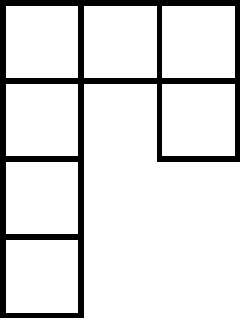
\includegraphics[height=3.2cm,width=2.5cm]{Net-D-19-5}
\end{figure}
\begin{answer}
	\begin{align*}
&\text{ Number of rectangles having length one unit and width two or three or four units $=7$}\\
&\text{	Number of rectangles having length three units and width one units $=2$}\\
&\text{	Number of rectangles having length three units and width one units $=1$}\\
&\text{	Hence total number of non-square rectangles $=7+2+1=10$}\\
	\end{align*}
	So the correct answer is \textbf{Option (c)}
\end{answer}
\item  The mean of a set of 10 numbers is $M$. By combining with it a second set of $M$ numbers, the mean of the combined set becomes 10 . What is the sum of the second set of numbers?
 \begin{tasks}(4)
	\task[\textbf{a.}]$10 M-1$
	\task[\textbf{b.}]$10 M+1$
	\task[\textbf{c.}]20
	\task[\textbf{d.}] 100
\end{tasks}
\begin{answer}
	\begin{align*}
&\text{ The sum of all numbers in the first set }=10 \times M=10 M\\
	&\text{Te sum of numbers in the combined set }=(10+M) \times 10=100+10 M\\
	&\text{ sum of second set of numbers}\\
	&\text{$=$ sum of numbers in combined set $-$ sum of numbers in first set }\\
	&=100+10 M-10 M=100
	\end{align*}
		So the correct answer is \textbf{Option (d)}
\end{answer}
\item Karan's house is $20 m$ to the east of Rahul's house. Mehul's house is $25 m$ to the NorthEast of Rahul's house. With respect to Mehul's house in which direction is Karan's house?
 \begin{tasks}(4)
	\task[\textbf{a.}]East
	\task[\textbf{b.}] South
	\task[\textbf{c.}]North-East
	\task[\textbf{d.}]  West
\end{tasks}
\begin{answer}$\left. \right. $
	\begin{figure}[H]
		\centering
		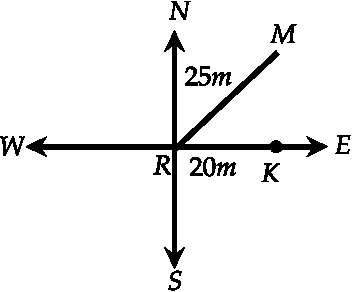
\includegraphics[height=3cm,width=3.5cm]{Net-D-19-6}
	\end{figure}
	\begin{align*}
	\intertext{ Mehul's house is $\frac{25}{\sqrt{2}} m$ to the East of Rahul's house and $\frac{25}{\sqrt{2}} m$ to the north of Rahul's house. Hence with respect to
		Mehul's house Karan house is in the South-East direction.
		None of the given options have this answer. So all of them are wrong.}
	\end{align*}
		So the correct answer is \textbf{Option (b)}
\end{answer}
\item A four-wheeled cart is going around a circular track. Which of the following statements is correct, if the four wheels are free to rotate independent of each other and the cart negotiates the track stably?
 \begin{tasks}(1)
	\task[\textbf{a.}] All wheels rotate at the same speed
	\task[\textbf{b.}] The four wheels have different speeds each
	\task[\textbf{c.}]The wheels closer to the inside of the track move slower than the outer-side wheels
	\task[\textbf{d.}]The wheels closer to the inside of the track move faster than the outer-side wheels	 
\end{tasks}	
\begin{answer}
 We consider that the angular speed of all parts of the car is uniform, call it $\omega$.\\
		Suppose that two types closer to the centre of the track are at a distance of $r_{1}$ from centre.
		Also suppose that the two types that are farther from the centre of track are at a distance $r_{2}$ from the centre. Clearly $r_{2}>r_{1}$\\
	Speed of wheels closer to the inside of track $=\omega r_{1}$\\
	Speed of wheels farther away from the track $=\omega r_{2}$\\
	Since $r_{2}>r_{1} \Rightarrow \omega r_{2}>\omega r_{1}$
	\begin{figure}[H]
		\centering
		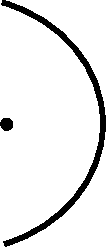
\includegraphics[height=2cm,width=0.8cm]{Net-D-19-7}
	\end{figure}
			So the correct answer is \textbf{Option (c)}
\end{answer}
\section{PART B}
\item The angular frequency of oscillation of a quantum harmonic oscillator in two dimensions is $\omega$. If it is in contact with an external heat bath at temperature $T$, its partition function is (in the following $\beta=\frac{1}{k_{B} T}$ )
 \begin{tasks}(2)
	\task[\textbf{a.}]$\frac{e^{2 \beta \hbar \omega}}{\left(e^{2 \beta \hbar \omega}-1\right)^{2}}$
	\task[\textbf{b.}]$\frac{e^{\beta \hbar \omega}}{\left(e^{\beta \hbar \omega}-1\right)^{2}}$
	\task[\textbf{c.}]$\frac{e^{\beta \hbar \omega}}{e^{\beta \hbar \omega}-1}$
	\task[\textbf{d.}] $\frac{e^{2 \beta \hbar \omega}}{e^{2 \beta \hbar \omega}-1}$v$\frac{e^{2 \beta \hbar \omega}}{e^{2 \beta \hbar \omega}-1}$
\end{tasks}
\begin{answer}
	\begin{align*}
	E_{n}&=(n+1) \hbar \omega \quad n=n_{x}+n_{y}
\text{	(2D Harmonic Oscillator)}\\
z&=\sum_{n=0}^{\infty}(n+1) e^{-(n+1) \hbar \omega} \text { degeneracy }=(n+1)\\
z&=e^{-\hbar \omega}+2 e^{-2 \hbar \omega}+3 e^{-3 \hbar \omega}+\ldots\\
z&=\frac{e^{-\beta \hbar \omega}}{1-e^{-\beta \hbar \omega}}+\frac{e^{-\beta 2 \hbar \omega}}{\left(1-e^{-\beta \hbar \omega}\right)^{2}}=\frac{e^{-\beta \hbar \omega}\left(1-e^{-\beta \hbar \omega}\right)+e^{-\beta 2 \hbar \omega}}{\left(1-e^{-\beta \hbar \omega}\right)^{2}}\\
&=\frac{e^{-\beta \hbar \omega}-e^{-2 \beta \hbar \omega}+e^{-\beta \hbar \omega}}{\left(1-e^{-\beta \hbar \omega}\right)^{2}}=\frac{e^{-\beta \hbar \omega}}{e^{-2 \beta \hbar \omega}\left(e^{\beta \hbar \omega}-1\right)^{2}}=\frac{e^{\beta \hbar \omega}}{\left(e^{\beta \hbar \omega}-1\right)^{2}}\\
\text { Note: } S_{n}&=a b+(a+d) b r+(a+2 d) b r^{2}+\ldots\\
S_{\infty}&=\frac{a b}{1-r}+\frac{d b r}{(1-r)^{2}}
	\end{align*}
		So the correct answer is \textbf{Option (b)}
\end{answer}
\item A student measures the displacement $x$ from the equilibrium of a stretched spring and reports it be $100 \mu \mathrm{m}$ with a $1 \%$ error. The spring constant $k$ is known to be $10 \mathrm{~N} / \mathrm{m}$ with $0.5 \%$ error. The percentage error in the estimate of the potential energy $V=\frac{1}{2} k x^{2}$ is
 \begin{tasks}(4)
	\task[\textbf{a.}]$0.8 \%$
	\task[\textbf{b.}] $2.5 \%$
	\task[\textbf{c.}] $1.5 \%$
	\task[\textbf{d.}] $3.0 \%$ 
\end{tasks}
\begin{answer}
	\begin{align*}
	\text { Percentage error in potential energy } V&=\frac{1}{2} k x^{2}\\
	\frac{\Delta V}{V} \%&=\frac{\Delta K}{K} \%+\frac{2 \Delta x}{x} \%\\
\text{	Given }\frac{\Delta K}{K} \%&=0.5 \%\text{ and }\frac{\Delta x}{x} \%=1 \%\\
	\therefore \quad \frac{\Delta V}{V} \%&=0.5 \%+2 \times 1 \%=2.5 \%
	\end{align*}
		So the correct answer is \textbf{Option (b)}
\end{answer}
\item The Hamiltonian of two interacting particles one with spin 1 and the other with spin $\frac{1}{2}$ is given by $H=A \vec{S}_{1} \cdot \vec{S}_{2}+B\left(S_{1 x}+S_{2 x}\right)$, where $\vec{S}_{1}$ and $\vec{S}_{2}$ denote the spin operators of the first and second particles, respectively and $A$ and $B$ are positive constants. The largest eigenvalue of this Hamiltonian is
 \begin{tasks}(2)
	\task[\textbf{a.}] $\frac{1}{2}\left(A \hbar^{2}+3 B \hbar\right)$
	\task[\textbf{b.}]$3 A \hbar^{2}+B \hbar$
	\task[\textbf{c.}] $\frac{1}{2}\left(3 A \hbar^{2}+B \hbar\right)$
	\task[\textbf{d.}]  $A \hbar^{2}+3 B \hbar$	
\end{tasks}
\begin{answer}
	\begin{align*}
	H&=A \vec{S}_{1} \cdot \vec{S}_{2}+B\left(S_{1 x}+S_{2 x}\right)\\
	S_{1}&=1 S_{2}=\frac{1}{2} \quad S=\frac{3}{2}, \frac{1}{2} \\
	H&=A \frac{|S|^{2}-\left|S_{1}\right|^{2}-\left|S_{2}\right|^{2}}{2}+B\left(S_{1 x}+S_{2 x}\right)\\
	\text { For largest eigen value for } s&=\frac{3}{2} \Rightarrow|S|=\frac{3}{2}\left(\frac{3}{2}+1\right) \hbar^{2}=\frac{15}{4} \hbar^{2}\\
	\left|S_{1}\right|^{2}&=1(1+1) \hbar^{2}=2 \hbar^{2} \\
	\left|S_{2}\right|^{2}&=\frac{1}{2}\left(\frac{1}{2}+1\right) \hbar^{2}=\frac{3}{4} \hbar^{2}\\
	S_{1 x}&=\hbar \quad S_{2 x}=\frac{\hbar}{2}\\
	H&=A \frac{\frac{15}{4} \hbar^{2}-2 \hbar^{2}-\frac{3}{4} \hbar^{2}}{2}+B\left(\hbar+\frac{\hbar}{2}\right) \\
	&=A \frac{(15-11) \hbar^{2}}{8}+\frac{3 B \hbar}{2}=A \frac{4}{8} \hbar^{2}+\frac{3 B \hbar}{2}=\frac{1}{2}\left(A \hbar^{2}+3 B \hbar\right)
	\end{align*}
		So the correct answer is \textbf{Option (a)}
\end{answer}
\item  Consider the set of polynomials $\left\{x(t)=a_{0}+a_{1} t+\ldots+a_{n-1} t^{n-1}\right\}$ in $t$ of degree less than $n$, such that $x(0)=0$ and $x(1)=1$. This set
 \begin{tasks}(1)
	\task[\textbf{a.}]Constitutes a vector space of dimension $n$
	\task[\textbf{b.}]Constitutes a vector space of dimension $n-1$
	\task[\textbf{c.}]Constitutes a vector space of dimension $n-2$
	\task[\textbf{d.}]Does not constitute a vector space	
\end{tasks}
\begin{answer}
	\begin{align*}
	x(t)&=a_{0}+a_{1} t+a_{2} t^{2}+\ldots+a_{n-1} y^{n-1}\\
	x(0)&=0 \\
	0&=a_{0} \\
	x(t)&=a_{1} t+a_{2} t^{2}+\ldots a_{n-1} t^{n-1}\\
\text{	also, }x(1)&=1\\
	1&=a_{1}+a_{2}+\ldots+a_{n-1}\\
	t, t^{2}, t^{3},& \ldots \text { will make basis vector if }\\
	c_{1} t&+c_{2} t^{2} c_{3} t^{3}+\ldots .=0\\
\text{	If }c_{1}&=c_{2}=c_{3}=\ldots=0\\
&\text{Which is contradicting with (i)}\\
&\text{So, it does not constitute a vector space. For our case if $a_1=a_2=.....=0$}\\
&\text{Its summation can't be }=1
	\end{align*}
		So the correct answer is \textbf{Option (d)}
\end{answer}
\item Consider black body radiation in thermal equilibrium contained in a two-dimensional box. The dependence of the energy density on the temperature $T$ is
 \begin{tasks}(4)
	\task[\textbf{a.}] $T^{3}$
	\task[\textbf{b.}]$T$
	\task[\textbf{c.}] $T^{2}$
	\task[\textbf{d.}] $T^{4}$
\end{tasks}
\begin{answer}
	\begin{align*}
	\text{The energy density at the temperature $T$ is,}
	\intertext {Energy density for $2 D$ photon, $u=\frac{2 \zeta(3)\left(k_{B} T\right)^{3}}{\hbar c^{2} \pi}, \zeta(s)=1+\frac{1}{2^{2}}+\frac{1}{3^{3}}+\ldots$, Riemann Zeta function $u \propto T^{3}$}
	\end{align*}
		So the correct answer is \textbf{Option (a)}
\end{answer}
\item The energy eigenvalues of a particle of mass $m$, confined to a rigid one-dimensional box of width $L$, are $E_{n}(n=1,2, \ldots)$. If the walls of the box are moved very slowly toward each other, the rate of change of time-dependent energy $\frac{d E_{2}}{d t}$ of the first excited state is
 \begin{tasks}(4)
	\task[\textbf{a.}]$\frac{E_{2}}{L} \frac{d L}{d t}$
	\task[\textbf{b.}]$\frac{2 E_{2}}{L} \frac{d L}{d t}$
	\task[\textbf{c.}]$-\frac{2 E_{2}}{L} \frac{d L}{d t}$
	\task[\textbf{d.}]$-\frac{E_{1}}{L} \frac{d L}{d t}$ 
\end{tasks}
\begin{answer}
	\begin{align*}
	E_{2}&=\frac{4 \pi^{2} \hbar^{2}}{2 m L^{2}} \Rightarrow \frac{d E_{2}}{d t}=-2 \frac{4 \pi^{2} \hbar^{2}}{2 m L^{3}} \frac{d L}{d t}=\frac{-2}{L} E_{2} \frac{d L}{d t}\\
	\frac{d E_{2}}{d t}&=\frac{-2 E_{2}}{L} \frac{d L}{d t}
	\end{align*}
		So the correct answer is \textbf{Option (c)}
\end{answer}
\item A ball, initially at rest, is dropped from a height $h$ above the floor bounces again and again vertically. If the coefficient of restitution between the ball and the floor is $0.5$, the total distance traveled by the ball before it comes to rest is
 \begin{tasks}(4)
	\task[\textbf{a.}]$\frac{8 h}{3}$
	\task[\textbf{b.}]$\frac{5 h}{3}$
	\task[\textbf{c.}] $3 h$
	\task[\textbf{d.}] $2 h$
\end{tasks}
\begin{answer}
	\begin{align*}
	v&=\sqrt{2 g h} \text { and } v_{1}=e \sqrt{2 g h}\\
	0&=(e v)^{2}-2 g h_{1} \Rightarrow h_{1}=\frac{e^{2} \times 2 g h}{2 g}=e^{2} h\\
	\text { Similarly, } h_{2}&=e^{4} h\\
	H&=h+2 h_{1}+2 h_{2}+\ldots \infty=h+2\left(e^{2} h+e^{4} h+\ldots \infty\right) \\
	&=h+2 e^{2} h\left(\frac{1}{1-e^{2}}\right)=h \times\left(\frac{1+e^{2}}{1-e^{2}}\right)\\
	\text { Put } e&=\frac{1}{2}=0.5=h \times\left(\frac{1+0.25}{1-0.25}\right)=h \times \frac{125}{75}=\frac{5 h}{3}
	\end{align*}
		So the correct answer is \textbf{Option (b)}
\end{answer}
\item Two spin $\frac{1}{2}$ fermions of mass $m$ are confined to move in a one-dimensional infinite potential well of width $L$. If the particles are known to be in a spin triplet state, the ground state energy of the system (in units of $\frac{\hbar^{2} \pi^{2}}{2 m L^{2}}$ ) is
 \begin{tasks}(4)
	\task[\textbf{a.}]8
	\task[\textbf{b.}]2
	\task[\textbf{c.}]3
	\task[\textbf{d.}] 5
\end{tasks}
\begin{answer}
	\begin{align*}
	\intertext{Solution: If probability in triplet state means $S_{1 z}=\frac{1}{2}$ and $S_{2 z}=\frac{1}{2}$. So one electron in $n=1$ state and another in $n=2$ state. So ground state energy of configuration is}
	\left(1^{2}+2^{2}\right) \frac{\pi^{2} \hbar^{2}}{2 m L^{2}}&=\frac{5 \pi^{2} \hbar^{2}}{2 m L^{2}}
	\end{align*}
		So the correct answer is \textbf{Option (d)}
\end{answer}
\item  The figure below shows a 2-bit simultaneous analog-to-digital (A/D) converter operating in the voltage range 0 to $V_{0}$. The output of the comparators are $C_{1}, C_{2}$ and $C_{3}$ with the reference inputs $V_{0} / 4, V_{0} / 2$ and $3 V_{0} / 4$, respectively. The logic expression for the output corresponding to the less significant bit is	
 \begin{tasks}(2)
	\task[\textbf{a.}]$C_{1} C_{2} C_{3}$
	\task[\textbf{b.}]$C_{2} \bar{C}_{3}+\bar{C}_{1}$
	\task[\textbf{c.}]$C_{1} \bar{C}_{2}+C_{3}$
	\task[\textbf{d.}] $C_{2} \bar{C}_{3}+C_{2}$	
\end{tasks}
\begin{figure}[H]
	\centering
	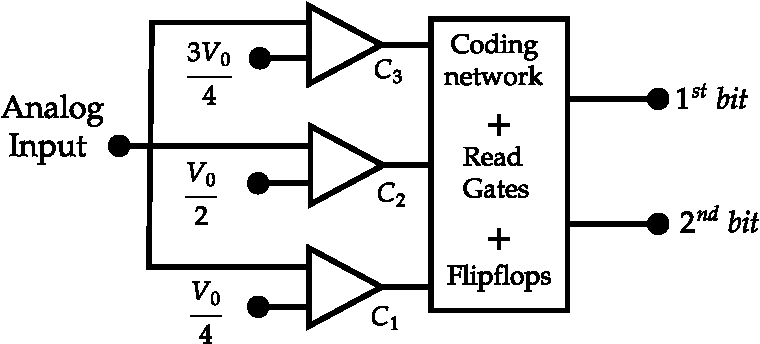
\includegraphics[height=3.5cm,width=7cm]{Net-D-19-8}
\end{figure}
\begin{answer}
	\begin{align*}
	\text { Least significant bit is }(0,1) \text { i.e. } C_{1} \text { will be selected and } C_{2}&=0, C_{3}=0\\
	\text { So output }=C_{1} \bar{C}_{2}+C_{3}=C_{1} \cdot \overline{0}+0&=C_{1}
	\end{align*}
		So the correct answer is \textbf{Option (c)}
\end{answer}
\item The $y z$ - plane at $x=0$ carries a uniform surface charge density $\sigma$. A unit point charge is moved from a point $(\delta, 0,0)$ on one side of the plane to a point $(-\delta, 0,0)$ on the other side. If $\delta$ is an infinitesimally small positive number, the work done in moving the charge is
 \begin{tasks}(4)
	\task[\textbf{a.}]0
	\task[\textbf{b.}]$\frac{\sigma}{\varepsilon_{0}} \delta$
	\task[\textbf{c.}]$-\frac{\sigma}{\varepsilon_{0}} \delta$
	\task[\textbf{d.}]$\frac{2 \sigma}{\varepsilon_{0}} \delta$ 
\end{tasks}
\begin{answer}
	\begin{align*}
	\text { Work done }& q[V(b)-V(a)]\\
	\text { Since work done }&\text{depends on potential difference between two points, }\\
\text{	So }W&=0
\text{	( Potential = constant )}
	\end{align*}
	So the correct answer is \textbf{Option (a)}
\end{answer}
\item A circular conducting wire loop is placed close to a solenoid as shown in the figure below. Also shown is the current through the solenoid as a function of time.	
\begin{figure}[H]
	\centering
	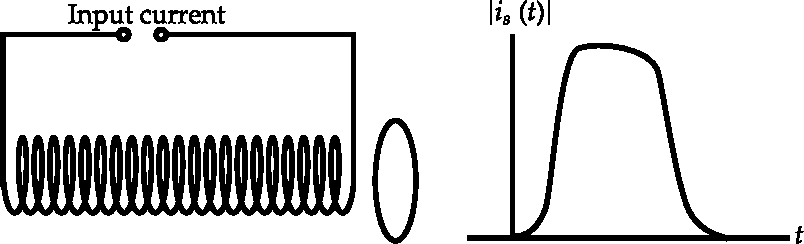
\includegraphics[height=2.5cm,width=8cm]{Net-D-19-9}
\end{figure}
The magnitude $|i(t)|$ of the induced current in the wire loop, as a function of time $t$, is best represented as
 \begin{tasks}(2)
	\task[\textbf{a.}]
	\begin{figure}[H]
		\centering
		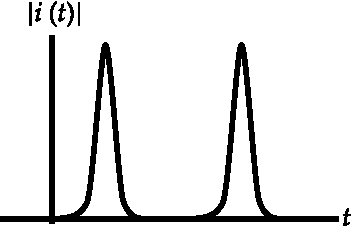
\includegraphics[height=3cm,width=5cm]{Net-D-19-10}
	\end{figure}
	\task[\textbf{b.}]
		\begin{figure}[H]
		\centering
		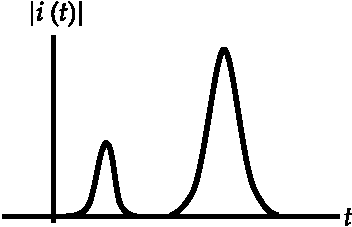
\includegraphics[height=3cm,width=5cm]{Net-D-19-11}
	\end{figure}
	\task[\textbf{c.}]
		\begin{figure}[H]
		\centering
		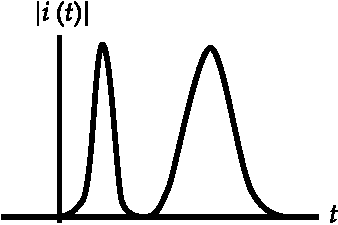
\includegraphics[height=3cm,width=5cm]{Net-D-19-12}
	\end{figure}
	\task[\textbf{d.}] 
		\begin{figure}[H]
		\centering
		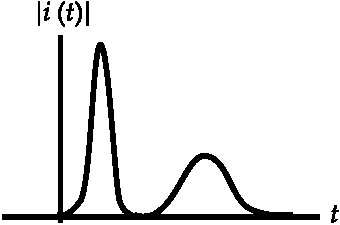
\includegraphics[height=3cm,width=5cm]{Net-D-19-13}
	\end{figure}
\end{tasks}
\begin{answer}
	\begin{align*}
	\text { Induced e.m.f } \varepsilon&=-\frac{d \phi}{d t}, \quad|l(t)|=\frac{|\varepsilon|}{R} \propto\left|\frac{d l s}{d t}\right|\\
	\intertext{So when current increases, $|l(t)|$ will increase and when it will decrease $|l(t)|$ will decrease.}
	\end{align*}
		So the correct answer is \textbf{Option (d)}
\end{answer}
\item A mole of gas at initial temperature $T_{i}$ comes into contact with a heat reservoir at temperature $T_{f}$ and the system is allowed to reach equilibrium at constant volume. If the specific heat of the gas is $C_{V}=\alpha T$, where $\alpha$ is a constant, the total change in entropy is
 \begin{tasks}(2)
	\task[\textbf{a.}]zero
	\task[\textbf{b.}] $\alpha\left(T_{f}-T_{i}\right)+\frac{\alpha}{2 T_{f}}\left(T_{f}-T_{i}\right)^{2}$
	\task[\textbf{c.}] $\alpha\left(T_{f}-T_{i}\right)$
	\task[\textbf{d.}]$\alpha\left(T_{f}-T_{i}\right)+\frac{\alpha}{2 T_{f}}\left(T_{f}^{2}-T_{i}^{2}\right)$
\end{tasks}
\begin{answer}$\left. \right. $
	\begin{figure}[H]
		\centering
		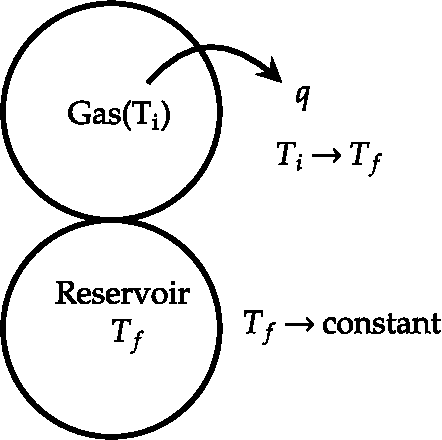
\includegraphics[height=3.5cm,width=3.5cm]{Net-D-19-14}
	\end{figure}
	\begin{align*}
	\text{Change in entropy of gas}\\
	T d s&=C_{V} d T+P d V, \mathrm{dV}=0 \\
	T d s&=\alpha T d T \\
	\Delta s_{g a s}&=\alpha\left[T_{f}-T_{i}\right]\\
	\text{Change in entropy of reservoir }&\text{(at constant temperature $T_f$)}\\
	T_{f} d s&=\alpha T d T \qquad d Q=\alpha T d T\\
	T_{f} \Delta s_{\mathrm{Res}}&=\left.\alpha \frac{T^{2}}{2}\right|_{T_{i}} ^{T_{f}}=\frac{\alpha}{2}\left[T_{f}^{2}-T_{i}^{2}\right] \\
	\Delta s_{\mathrm{Res}}&=\frac{\alpha}{2 T_{f}}\left[T_{f}^{2}-T_{i}^{2}\right], \quad \Delta s_{\text {total }}=\alpha\left[T_{f}-T_{i}\right]+\frac{\alpha}{2 T_{f}}\left[T_{f}^{2}-T_{i}^{2}\right]
	\end{align*}
		So the correct answer is \textbf{Option (d)}
\end{answer}
\item An ideal Carnot engine extracts $100 \mathrm{~J}$ from a heat source and dumps $40 \mathrm{~J}$ to a heat sink at $300 \mathrm{~K}$. The temperature of the heat source is
 \begin{tasks}(4)
	\task[\textbf{a.}]$600 \mathrm{~K}$
	\task[\textbf{b.}]$700 \mathrm{~K}$
	\task[\textbf{c.}] $750 \mathrm{~K}$
	\task[\textbf{d.}] $650 \mathrm{~K}$
\end{tasks}
\begin{answer}
	\begin{align*}
	Q_{1}&=100 \mathrm{~J}, Q_{2}=40 \mathrm{~J}\\
	T_{1}&=? \quad T_{2}=300 \mathrm{~K} \\
	\frac{Q_{1}}{Q_{2}}&=\frac{T_{1}}{T_{2}} \Rightarrow \frac{100}{40}=\frac{T_{1}}{300} \Rightarrow T_{1}=\frac{100 \times 300}{40} \\
	\Rightarrow T_{1}&=750 \mathrm{~K}
	\end{align*}
		So the correct answer is \textbf{Option (c)}
\end{answer}
\item A block of mass $m$, attached to a spring, oscillates horizontally on a surface. The coefficient of friction between the block and the surface is $\mu$. Which of the following trajectories best describes the motion of the block in the phase space ( $x p_{x}$-plane)?	
\begin{figure}[H]
	\centering
	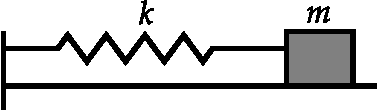
\includegraphics[height=1cm,width=4cm]{Net-D-19-15}
\end{figure}
 \begin{tasks}(2)
	\task[\textbf{a.}]
	\begin{figure}[H]
		\centering
		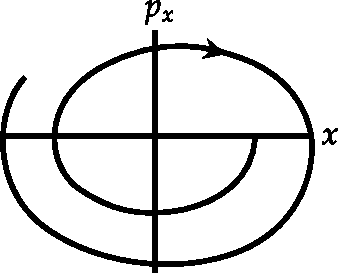
\includegraphics[height=2cm,width=3cm]{Net-D-19-16}
	\end{figure}
	\task[\textbf{b.}]
		\begin{figure}[H]
		\centering
		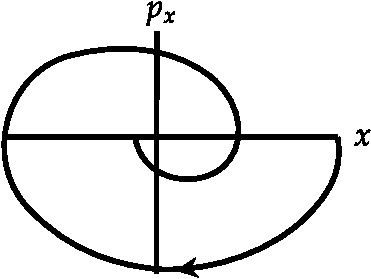
\includegraphics[height=2cm,width=3cm]{Net-D-19-17}
	\end{figure}
	\task[\textbf{c.}]
		\begin{figure}[H]
		\centering
		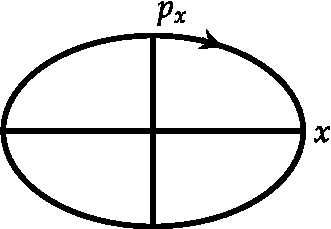
\includegraphics[height=2cm,width=3cm]{Net-D-19-18}
	\end{figure}
	\task[\textbf{d.}] 
		\begin{figure}[H]
		\centering
		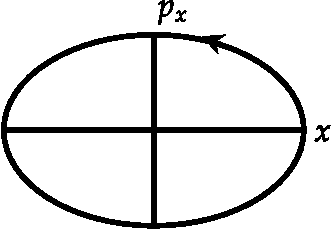
\includegraphics[height=2cm,width=3cm]{Net-D-19-19}
	\end{figure}
\end{tasks}
\begin{answer}
 Due to friction amplitude and momentum of oscillation continuously decreases. So option (b) is correct.
 \begin{figure}[H]
 	\centering
 	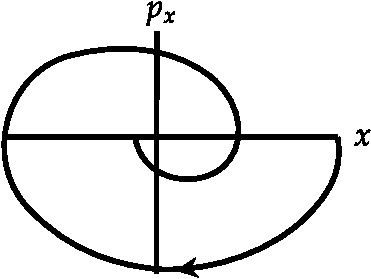
\includegraphics[height=2cm,width=3cm]{Net-D-19-17}
 \end{figure}
	So the correct answer is \textbf{Option (b)}
\end{answer}
\item Let $C$ be the circle of radius $\frac{\pi}{4}$ centered at $z=\frac{1}{4}$ in the complex $z$-plane that is traversed counter-clockwise. The value of the contour integral $\oint_{C} \frac{z^{2}}{\sin ^{2} 4 z} d z$ is
 \begin{tasks}(4)
	\task[\textbf{a.}]0
	\task[\textbf{b.}]$\frac{i \pi^{2}}{4}$
	\task[\textbf{c.}] $\frac{i \pi^{2}}{16}$
	\task[\textbf{d.}] $\frac{i \pi}{4}$
\end{tasks}
\begin{answer}$\left. \right. $
	\begin{figure}[H]
		\centering
		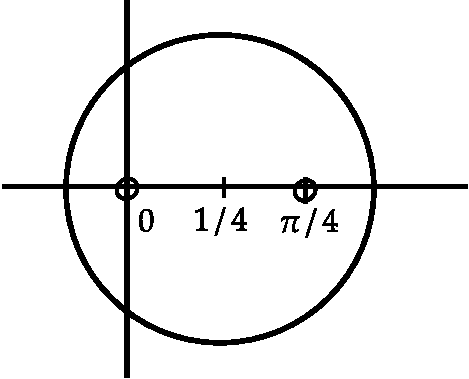
\includegraphics[height=3.5cm,width=4.5cm]{Net-D-19-21}
	\end{figure}
	\begin{align*}
	f(z)&=\left(\frac{\pi}{\sin 4 z}\right)^{2}\\
	z_{0}&=0, \frac{\pi}{4}\text{ are poles}\\
	4 z&=n \pi, z=0, \frac{\pi}{4}\\
	\text{Others are outside the contour.}\\
	\text { Residue at } z&=0 \text { is }\left[\frac{\pi}{4 z-\frac{4^{3} z^{3}}{3 !}+\ldots}\right]^{2}\\
	&=\left[\frac{1}{4-\frac{4^{3} z^{2}}{3 !}+\ldots}\right]^{2}
	\text{No terms for $\frac{1}{z}, b_{1}=0$}\\
	&=\left[4-\frac{4^{3} z^{2}}{3 !}+\ldots\right]^{-2}\\
\text{	Residue for }z&=\frac{\pi}{4}\\
	z-\frac{\pi}{4}&=t\\
	\sin (4 t+\pi)&=-\sin 4 t
\text{	(But square so no effect)}\\
&\left[\frac{t+\frac{\pi}{4}}{\sin 4\left(t+\frac{\pi}{4}\right)}\right]^{2}\\
\left(\frac{t+\frac{\pi}{4}}{\sin 4 t}\right)^{2}&=\frac{t^{2}+\frac{\pi^{2}}{4}+2 t \cdot \frac{\pi}{4}}{\sin ^{2} 4 t} \\
\frac{\pi}{2} \frac{t}{16 t^{2}[1-\ldots .]^{2}}&=\frac{\pi}{32 t}[1-\ldots .]^{-2} \quad \text{from first term}\\
b_{1}&=\frac{\pi}{32}\\
\oint_{C} \frac{z^{2}}{\sin ^{2} 4 z} d z&=2 \pi i\left[0+\frac{\pi}{32}\right]=\frac{i \pi^{2}}{16}
	\end{align*}
	So the correct answer is \textbf{Option (c)}
\end{answer}
\item If the rank of an $n \times n$ matrix $A$ is $m$, where $m$ and $n$ are positive integers with $1 \leq m \leq n$, then the rank of the matrix $A^{2}$ is
 \begin{tasks}(4)
	\task[\textbf{a.}]$m$
	\task[\textbf{b.}]$m-1$
	\task[\textbf{c.}]$2 m$
	\task[\textbf{d.}]$m-2$ 
\end{tasks}
\begin{answer}
	\begin{align*}
	\text{Let }\sigma_{1}&=\left[\begin{array}{ll}0 & 1 \\ 1 & 0\end{array}\right]_{\substack{2 \times 2 \\ n=2}}=A \quad m=2\\
	1 \leq 2 \leq 2 &\qquad 1 \leq m \leq n\\
	A^{2}&=\left[\begin{array}{ll}
	1 & 0 \\
	0 & 1
	\end{array}\right]_{2 \times 2} m=2\\
	\text { (b), (c), (d) }&\text{can't be correct so option (a) is correct. }
	\end{align*}
		So the correct answer is \textbf{Option (a)}
\end{answer}
\item A particle of mass $m$ is confined to a box of unit length in one dimension. It is described by the wavefunction $\psi(x)=\sqrt{\frac{8}{5}} \sin \pi x(1+\cos \pi x)$ for $0 \leq x \leq 1$ and zero outside this interval. The expectation value of energy in this state is
 \begin{tasks}(4)
	\task[\textbf{a.}] $\frac{4 \pi^{2}}{3 m} \hbar^{2}$
	\task[\textbf{b.}]$\frac{4 \pi^{2}}{5 m} \hbar^{2}$
	\task[\textbf{c.}]$\frac{2 \pi^{2}}{5 m} \hbar^{2}$
	\task[\textbf{d.}]  $\frac{8 \pi^{2}}{5 m} \hbar^{2}$
\end{tasks}
\begin{answer}
	\begin{align*}
	&\sqrt{\frac{8}{5}} \sin \pi x(1+\cos \pi x)\\
	&\sqrt{\frac{8}{5}} \sin \pi x+\sqrt{\frac{8}{5}} \sin \pi x \cos \pi x \\
	&\sqrt{\frac{8}{5}} \frac{1}{\sqrt{2}} \sqrt{\frac{2}{1}} \sin \pi x+\sqrt{\frac{8}{5}} \times \frac{1}{2} \times \frac{1}{\sqrt{2}} \sqrt{\frac{2}{1}} \sin 2 \pi x \\
	&\sqrt{\frac{4}{5}}\left|\phi_{1}\right\rangle+\sqrt{\frac{1}{5}}\left|\phi_{2}\right\rangle\\
	\langle E\rangle&=\frac{4}{5} \times E_{0}+\frac{1}{5} \times 4 E_{0}=2 \times \frac{4}{5} E_{0}=\frac{4 \pi^{2} \hbar^{2}}{5 m} \text { where } E_{0}=\frac{\pi^{2} \hbar^{2}}{2 m}
	\end{align*}
			So the correct answer is \textbf{Option (b)}
\end{answer}
\item In the circuit below, $D$ is an ideal diode, the source voltage $V_{S}=V_{0} \sin \omega t$ is a unit amplitude sine wave and $R_{S}=R_{L}$	
\begin{figure}[H]
	\centering
	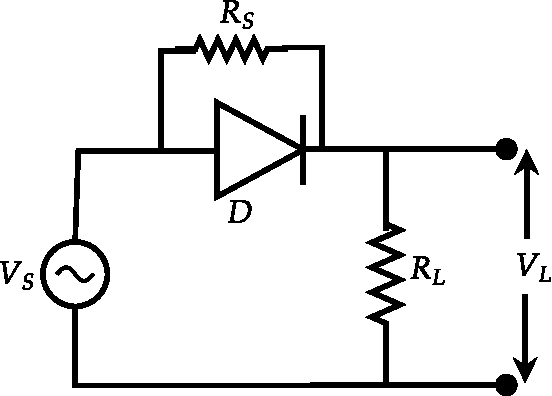
\includegraphics[height=3cm,width=4.5cm]{Net-D-19-22}
\end{figure}
The average output voltage, $V_{L}$, across the load resistor $R_{L}$ is
 \begin{tasks}(4)
	\task[\textbf{a.}] $\frac{1}{2 \pi} V_{0}$
	\task[\textbf{b.}] $\frac{3}{2 \pi} V_{0}$
	\task[\textbf{c.}]$3 V_{0}$
	\task[\textbf{d.}]$V_{0}$ 
\end{tasks}
\begin{answer}
	\begin{align*}
	\text { Positive half cycle } V_{L}&=V_{S}=V_{0} \sin \omega t\\
	\text{Negative half cycle }V_{L}&=\frac{V_{S}}{2}=\frac{V_{0}}{2} \sin \omega t\\
	V_{a v}&=\frac{1}{2 \pi}\left[\int_{0}^{\pi} V_{0} \sin \theta d \theta+\int_{\pi}^{2 \pi} \frac{V_{0}}{2} \sin \theta d \theta\right]=\frac{1}{2 \pi} V_{0}
	\end{align*}
		So the correct answer is \textbf{Option (a)}
\end{answer}
\item The normalized wavefunction of a particle in three dimensions is given by
$$
\psi(x, y, z)=N z \exp \left[-a\left(x^{2}+y^{2}+z^{2}\right)\right]
$$
where $a$ is a positive constant and $N$ is a normalization constant. If $L$ is the angular momentum operator, the eigenvalues of $L^{2}$ and $L_{z}$, respectively, are
 \begin{tasks}(4)
	\task[\textbf{a.}]$2 \hbar^{2}$ and $\hbar$
	\task[\textbf{b.}]$\hbar^{2}$ and 0
	\task[\textbf{c.}] $2 \hbar^{2}$ and 0
	\task[\textbf{d.}] $\frac{3}{4} \hbar^{2}$ and $\frac{1}{2} \hbar$
\end{tasks}
\begin{answer}
	\begin{align*}
	\psi(x, y, z)&=N z \exp \left[-a\left(x^{2}+y^{2}+z^{2}\right)\right]\\
	\psi(r, \theta, \phi)&=N r \cos \theta \exp (-r)^{2} \text { so } m=0, l=1\\
	L^{2}&=2 \hbar^{2} \text { and } L_{z}=0 \hbar
	\end{align*}
		So the correct answer is \textbf{Option (c)}
\end{answer}
\item The electric field of an electromagnetic wave is $\vec{E}=\hat{i} \sqrt{2} \sin (k z-\omega t) V m^{-1}$. The average flow of energy per unit area per unit time, due to this wave, is
 \begin{tasks}(4)
	\task[\textbf{a.}]$27 \times 10^{4} \mathrm{~W} / \mathrm{m}^{2}$
	\task[\textbf{b.}]$27 \times 10^{-4} \mathrm{~W} / \mathrm{m}^{2}$
	\task[\textbf{c.}]$27 \times 10^{-2} \mathrm{~W} / \mathrm{m}^{2}$
	\task[\textbf{d.}] $27 \times 10^{2} \mathrm{~W} / \mathrm{m}^{2}$
\end{tasks}
\begin{answer}
	\begin{align*}
	\langle\vec{S}\rangle&=\frac{E / t}{A}=I=\frac{1}{2} \epsilon_{0} E_{0}^{2} c\\
	\Rightarrow I&=\frac{1}{2} \times 8.86 \times 10^{-12}(\sqrt{2})^{2} \times 3 \times 10^{8}\\
	\Rightarrow I &\approx 27 \times 10^{-4} \mathrm{~W} / \mathrm{m}^{2}
	\end{align*}
		So the correct answer is \textbf{Option (b)}
\end{answer}
\item The energies available to a three state system are $0, E$ and $2 E$, where $E>0$. Which of the following graphs best represents the temperature dependence of the specific heat?
 \begin{tasks}(2)
	\task[\textbf{a.}]
	\begin{figure}[H]
		\centering
		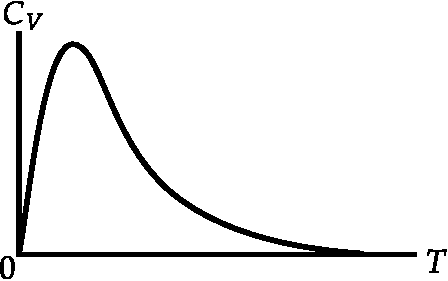
\includegraphics[height=2.5cm,width=4cm]{Net-D-19-23}
	\end{figure}
	\task[\textbf{b.}]
	\begin{figure}[H]
		\centering
		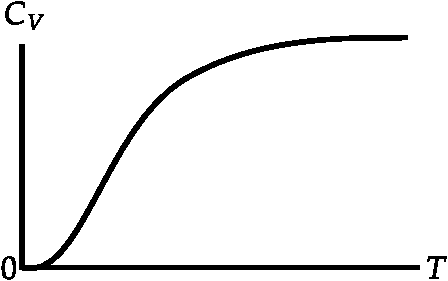
\includegraphics[height=2.5cm,width=4cm]{Net-D-19-24}
	\end{figure}
	\task[\textbf{c.}]
	\begin{figure}[H]
		\centering
		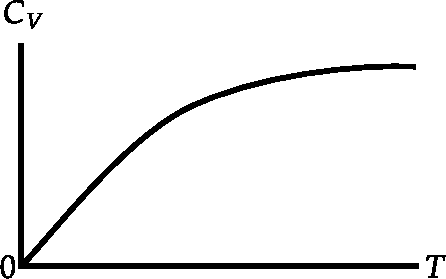
\includegraphics[height=2.5cm,width=4cm]{Net-D-19-25}
	\end{figure}
	\task[\textbf{d.}] 
	\begin{figure}[H]
		\centering
		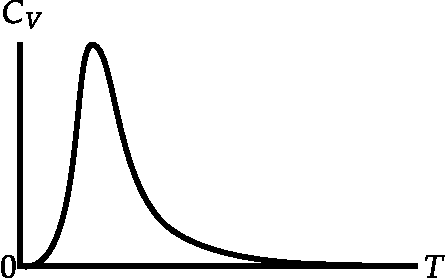
\includegraphics[height=2.5cm,width=4cm]{Net-D-19-26}
	\end{figure}
\end{tasks}	
\begin{answer}
	So the correct answer is \textbf{Option (d)}
\end{answer}
\item The values of $a$ and $b$ for which the force $F=\left(a x y+z^{3}\right) \hat{i}+x^{2} \hat{j}+b x z^{2} \hat{k}$ is conservative are
 \begin{tasks}(2)
	\task[\textbf{a.}]$a=2, b=3$
	\task[\textbf{b.}]$a=1, b=3$
	\task[\textbf{c.}]$a=2, b=6$
	\task[\textbf{d.}]$a=3, b=2$
\end{tasks}
\begin{answer}
	\begin{align*}
	\text { For conservative force } \vec{\nabla} \times \vec{F}&=0 \Rightarrow\left|\begin{array}{ccc}
	\hat{x} & \hat{y} & \hat{z} \\
	\frac{\partial}{\partial x} & \frac{\partial}{\partial y} & \frac{\partial}{\partial z} \\
	a x y+z^{3} & x^{2} & b x z^{2}
	\end{array}\right|=0\\
	\Rightarrow \hat{x}(0-0)-\hat{y}\left(b z^{2}-3 z^{2}\right)+\hat{z}(2 x-a x)&=0 \\
	\Rightarrow b-3=0 \text { and } z-a=0 \text { or } a=2, b=3
	\end{align*}
		So the correct answer is \textbf{Option (a)}
\end{answer}
\item A positively charged particle is placed at the origin (with zero initial velocity) in the presence of a constant electric and a constant magnetic field along the positive $z$ and $x$-directions, respectively. At large times, the overall motion of the particle is adrift along the
 \begin{tasks}(2)
	\task[\textbf{a.}] Positive $y$-direction
	\task[\textbf{b.}] Negative $z$ - direction
	\task[\textbf{c.}]Positive $z$ - direction
	\task[\textbf{d.}]  Negative $y$-direction
\end{tasks}
\begin{answer}
 Initially charged particle will experience electric force and will gain velocity then it will deflect in magnetic field $[\vec{F} \propto(\vec{v} \times B) \rightarrow \hat{y}]$.
 \begin{figure}[H]
 	\centering
 	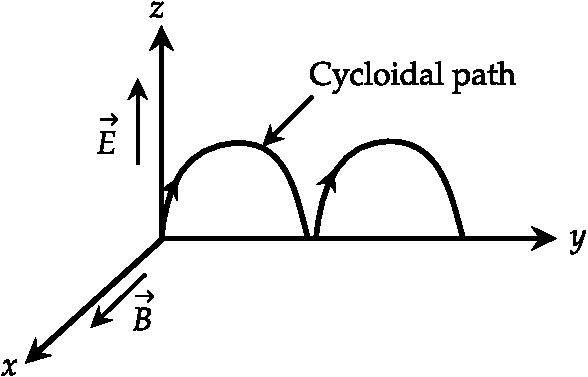
\includegraphics[height=3cm,width=5cm]{Net-D-19-27}
 \end{figure}
		So the correct answer is \textbf{Option (a)}
\end{answer}
\item A box contains 5 white and 4 black balls. Two balls are picked together at random from the box. What is the probability that these two balls are of different colours?
 \begin{tasks}(4)
	\task[\textbf{a.}] $\frac{1}{2}$
	\task[\textbf{b.}]$\frac{5}{18}$
	\task[\textbf{c.}]$\frac{1}{3}$
	\task[\textbf{d.}]  $\frac{5}{9}$
\end{tasks}
\begin{answer}
	\begin{align*}
	&\text { Probability that the two balls are of different colors }5 W, 4 B\\
	&=\frac{5 C_{1} \times 4 C_{1}}{9 C_{2}}=\frac{\frac{5 !}{4 ! \times 1 !} \times \frac{4 !}{3 ! \times 1 !}}{\frac{9 !}{7 ! \times 2 !}}=\frac{5 \times 4}{\frac{9 \times 8}{2}}=\frac{5}{9}
	\end{align*}
		So the correct answer is \textbf{Option (d)}
\end{answer}
\item Which of the following terms, when added to the Lagrangian $L(x, y, \dot{x}, \dot{y})$ of a system with two degrees of freedom will not change the equations of motion?
 \begin{tasks}(4)
	\task[\textbf{a.}]$x \ddot{x}-y \ddot{y}$
	\task[\textbf{b.}]$x \ddot{y}-y \ddot{x}$
	\task[\textbf{c.}]$x \dot{y}-y \dot{x}$
	\task[\textbf{d.}] $y \dot{x}^{2}+x \dot{y}^{2}$
\end{tasks}
\begin{answer}
	\begin{align*}
	L(x, y, \dot{x}, \dot{y})&\\
	\frac{d}{d t}\left(\frac{\partial L}{\partial \dot{x}}\right)-\frac{\partial L}{\partial x}&=0, \frac{d}{d t}\left(\frac{\partial L}{\partial \dot{y}}\right)-\frac{\partial L}{\partial y}=0 \\
	L^{\prime}&=L(x, y, \dot{x}, \dot{y})+x \ddot{y}-y \ddot{x} \\
	\frac{d^{\prime}}{d t^{\prime}}\left(\frac{\partial L^{\prime}}{\partial \dot{x}}\right)-\frac{\partial L^{\prime}}{\partial x}&=\frac{d}{d t}\left(\frac{\partial L}{\partial \dot{x}}\right)-\frac{\partial L}{\partial x}+\ddot{y}=0=0+\ddot{y}=0 \Rightarrow \dot{y}=c_{1} \\
	\frac{d}{d t}\left(\frac{\partial L}{\partial y}\right)-\frac{\partial L^{\prime}}{\partial y}&=\frac{d}{d t}\left(\frac{\partial L}{\partial \dot{y}}\right)-\frac{\partial L}{\partial y}+\ddot{x}=0=0-\ddot{x}=0 \Rightarrow \dot{x}=c_{2}
	\end{align*}
	So the correct answer is \textbf{Option (b)}
\end{answer}
(check question)	
\section{PART C}
\item The outermost shell of an atom of an element is $3 d^{3}$. The spectral symbol for the ground state is
 \begin{tasks}(4)
	\task[\textbf{a.}] ${ }^{4} F_{3 / 2}$
	\task[\textbf{b.}]${ }^{4} F_{9 / 2}$
	\task[\textbf{c.}]${ }^{4} D_{7 / 2}$
	\task[\textbf{d.}] ${ }^{4} D_{1 / 2}$
\end{tasks}
\begin{answer}
	\begin{align*}
	\text { For } d^{3}: &\quad M_{L}=-2-10+1+2\\
	\text{Highest }S&=\sum M_{S}=\frac{1}{2}+\frac{1}{2}+\frac{1}{2}=\frac{3}{2}\\
\text{	Highest }L&=\left|\sum M_{L}\right|=|-2-1+0|=3\\
\text{	Lowest }J&=|L-S|=\left|3-\frac{3}{2}\right|=\frac{3}{2}\\
\text{	Spectral term }&={ }^{2 S+1} L_{J}={ }^{4} F_{3 / 2}
	\end{align*}
		So the correct answer is \textbf{Option (a)}
\end{answer}
\item In a spectrum resulting from Raman scattering, let $I_{R}$ denote the intensity of Rayleigh scattering and $I_{S}$ and $I_{A S}$ denote the most intense Stokes line and the most intense antiStokes line, respectively. The correct order of these intensities is
 \begin{tasks}(2)
	\task[\textbf{a.}] $I_{S}>I_{R}>I_{A S}$
	\task[\textbf{b.}]$I_{R}>I_{S}>I_{A S}$
	\task[\textbf{c.}]$I_{A S}>I_{R}>I_{S}$
	\task[\textbf{d.}]$I_{R}>I_{A S}>I_{S}$ 
\end{tasks}
\begin{answer}$\left. \right. $
	\begin{figure}[H]
		\centering
		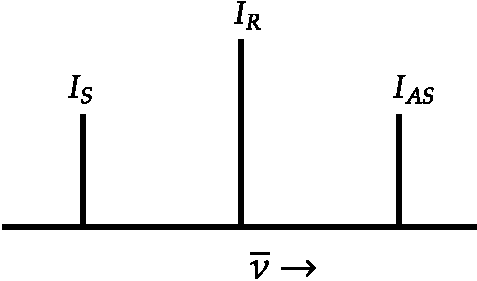
\includegraphics[height=2.8cm,width=5cm]{Net-D-19-28}
	\end{figure}
	 Intensity of Rayleigh line is always higher than intensity of stokes and Anti-stokes line.
	Whereas the intensity of stokes-line is lighter than anti-stokes line
	\begin{align*}
	\text { Thus } I_{R}>I_{S}>I_{A S}
	\end{align*}
	So the correct answer is \textbf{Option (b)}
\end{answer}
\item A particle hops randomly from a site to its nearest neighbour in each step on a square lattice of unit lattice constant. The probability of hopping to the positive $x$-direction is $0.3$, to the negative $x$-direction is $0.2$, to the positive $y$-direction is $0.2$ and to the negative $y$-direction is $0.3$. If a particle starts from the origin, its mean position after $N$ steps is
 \begin{tasks}(2)
	\task[\textbf{a.}] $\frac{1}{10} N(-\hat{i}+\hat{j})$
	\task[\textbf{b.}]$\frac{1}{10} N(\hat{i}-\hat{j})$
	\task[\textbf{c.}]$N(0.3 \hat{i}-0.2 \hat{j})$
	\task[\textbf{d.}]  $N(0.2 \hat{i}-0.3 \hat{j})$
\end{tasks}
\begin{answer}
	\begin{align*}
	&\left\langle r_{i}\right\rangle \sum_{i} p_{i} r_{i}\\
	&=0.3 \hat{i}-0.2 \hat{i}+0.2 j-0.3 \hat{j}=0.1 \hat{i}-0.1 \hat{j}\\
	\text{For $N$ steps, }&=\frac{N}{10}[\hat{i}-\hat{j}]
	\end{align*}
		So the correct answer is \textbf{Option (b)}
\end{answer}
\item Let $\hat{x}$ and $\hat{p}$ denote position and momentum operators obeying the commutation relation $[\hat{x}, \hat{p}]=i \hbar$. If $|x\rangle$ denotes an eigenstate of $\hat{x}$ corresponding to the eigenvalue $x$, then $e^{i a \hat{p} / \hbar}|x\rangle$ is	
 \begin{tasks}(1)
	\task[\textbf{a.}] an eigenstate of $\hat{x}$ corresponding to the eigenvalue $x$
	\task[\textbf{b.}] an eigenstate of $\hat{x}$ corresponding to the eigenvalue $(x+a)$
	\task[\textbf{c.}]an eigenstate of $\hat{x}$ corresponding to the eigenvalue $(x-a)$
	\task[\textbf{d.}] not an eigenstate of $\hat{x}$	
\end{tasks}
\begin{answer}
	\begin{align*}
	&e^{\frac{i a P}{\hbar}}|x\rangle\\
	&=\left[\sum_{n=0}^{\infty} \frac{1}{\lfloor n}\left(\frac{i a P}{\hbar}\right)^{n}\right]|x\rangle=\left[\sum_{n=0}^{\infty} \frac{1}{\lfloor n}(-a \nabla)^{n}\right]^{h}|x\rangle \\
	&=|x\rangle-a \vec{\nabla}|x\rangle+\frac{1}{\lfloor 2}(a \vec{\nabla})^{2}|x\rangle \ldots .=|x-a\rangle \\
	X|x-a\rangle&=(x-a)|x-a\rangle
	\end{align*}
		So the correct answer is \textbf{Option (c)}
\end{answer}
\item The strong nuclear force between a neutron and a proton in a zero orbital angular momentum state is denoted by $F_{n p}(r)$, where $r$ is the separation between them. Similarly, $F_{n n}(r)$ and $F_{p p}(r)$ denote the forces between a pair of neutrons and protons, respectively, in zero orbital momentum state. Which of the following is true on average if the inter-nucleon distance is $0.2 \mathrm{fm}<r<2 \mathrm{fm}$ ?
 \begin{tasks}(1)
	\task[\textbf{a.}]$F_{n p}$ is attractive for triplet spin state, and $F_{n n}, F_{p p}$ are always repulsive
	\task[\textbf{b.}]$F_{n n}$ and $F_{n p}$ are always attractive and $F_{p p}$ is repulsive in the triplet spin state
	\task[\textbf{c.}] $F_{p p}$ and $F_{n p}$ are always attractive and $F_{n n}$ is always repulsive
	\task[\textbf{d.}] All three forces are always attractive
\end{tasks}
\begin{answer}
	Inside the nucleus the interaction between neutron neutron and newtran-proton is always attractive due to nuclear force whereas between proton-proton it is repulusive due to coulombic interaction:\\
	Thus $F_{n n}$ and $F_{n p}$ are always attractive and $F_{p p}$ is repulsive\\
	So the correct answer is \textbf{Option (b)}
\end{answer}
\item The Hall coefficient for a semiconductor having both types of carriers is given as
$$
R_{H}=\frac{p \mu_{p}^{2}-n \mu_{n}^{2}}{|e|\left(p \mu_{p}+n \mu_{n}\right)^{2}}
$$
where $p$ and $n$ are the carrier densities of the holes and electrons, $\mu_{p}$ and $\mu_{n}$ are their respective mobilities. For a $p$ - type semiconductor in which the mobility of holes is less than that of electrons, which of the following graphs best describes the variation of the Hall coefficient with temperature?	
\begin{answer}
	 \begin{tasks}(2)
		\task[\textbf{a.}]
		\begin{figure}[H]
			\centering
			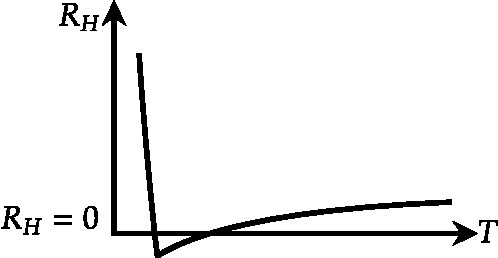
\includegraphics[height=2.5cm,width=4.5cm]{Net-D-19-29}
		\end{figure}
		\task[\textbf{b.}]
			\begin{figure}[H]
			\centering
			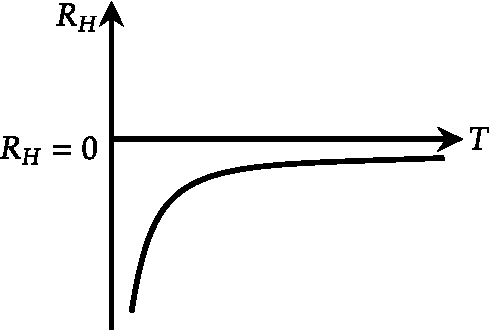
\includegraphics[height=2.5cm,width=4.5cm]{Net-D-19-30}
		\end{figure}
		\task[\textbf{c.}]
			\begin{figure}[H]
			\centering
			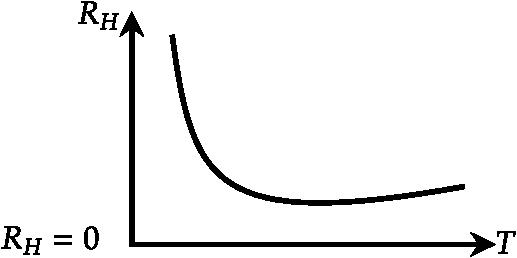
\includegraphics[height=2.5cm,width=4.5cm]{Net-D-19-31}
		\end{figure}
		\task[\textbf{d.}] 
			\begin{figure}[H]
			\centering
			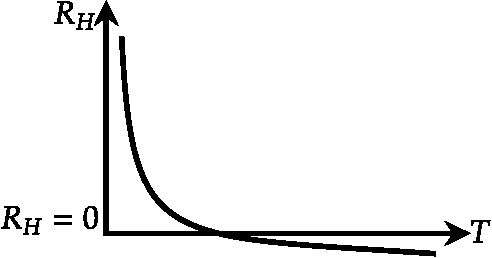
\includegraphics[height=2.5cm,width=4.5cm]{Net-D-19-32}
		\end{figure}
	\end{tasks}
	\begin{align*}
	&\text { Case I: At low temperature: } p>>n, \mu_{p}<\mu_{n}\\
	&\Rightarrow p \mu_{p}^{2}>n \mu_{n}^{2} \Rightarrow p \mu_{p}^{2}-n \mu_{n}^{2}>0 \\
	&\Rightarrow R_{H}=\text { Positive }\\\\
	&\text { Case II: At moderate temperature } \frac{p}{n}>1\\
	&\Rightarrow p \mu_{p}^{2} \approx n \mu_{n}^{2} \quad\left(\right.\text{ since }\mu_{p}<\mu_{n} )\\
	&\therefore R_{H} \simeq 0\\
	&\text { Case III: At high temperature } \frac{p}{n} \approx 1\\
	&\Rightarrow p \mu_{p}^{2}-n \mu_{n}^{2}<0 \quad\left(\right. \text{since }\left.\mu_{p}<\mu_{p}\right)\\
	&\therefore R_{H}<0
	\end{align*}
	Thus graph
	(d) correctly repeated the variation of $R_{H}$ with respect to temperature\\
	So the correct answer is \textbf{Option (d)}
\end{answer}
\item The generator of the infinitesimal canonical transformation $q \rightarrow q^{\prime}=(1+\epsilon) q$ and $p \rightarrow p^{\prime}=(1-\epsilon) p$ is
 \begin{tasks}(4)
	\task[\textbf{a.}]$q+p$
	\task[\textbf{b.}]$q p$
	\task[\textbf{c.}]$\frac{1}{2}\left(q^{2}-p^{2}\right)$
	\task[\textbf{d.}] $\frac{1}{2}\left(q^{2}+p^{2}\right)$
\end{tasks}
\begin{answer}
	\begin{align*}
	q \rightarrow q^{\prime}&=(1+\in) q\\
	p \rightarrow p^{\prime}&=(1-\epsilon) p\\
	\text{If $G$ is generator then }
	p^{\prime}-p&=\delta p_{j}=-\in \frac{\partial G}{\partial q_{j}} \Rightarrow p^{\prime}-p=-\in p\\
	q^{\prime}-q&=\delta q_{i}=\in \frac{\partial G}{\partial p_{j}} \Rightarrow q^{\prime}-q=\in p\\
	\text { We must check all options but if } G&=q p\\
	-\in \frac{\partial G}{\partial q}&=-\in p=\delta p \\
	\in \frac{\partial G}{\partial p}&=\in q=\delta q
	\end{align*}
		So the correct answer is \textbf{Option (b)}
\end{answer}
\item Assume that the noise spectral density, at any given frequency, in a current amplifier is independent of frequency. The bandwidth of measurement is changed from $1 \mathrm{~Hz}$ to $10 \mathrm{~Hz}$. The ratio $A / B$ of the RMS noise current before $(A)$ and after $(B)$ the bandwidth modification is
 \begin{tasks}(4)
	\task[\textbf{a.}]$1 / 10$
	\task[\textbf{b.}] $1 / \sqrt{10}$
	\task[\textbf{c.}]$\sqrt{10}$
	\task[\textbf{d.}]  10
\end{tasks}
\begin{answer}
		So the correct answer is \textbf{Option (b)}
\end{answer}
\item Let the normalized eigenstates of the Hamiltonian $H=\left(\begin{array}{ccc}2 & 1 & 0 \\ 1 & 2 & 0 \\ 0 & 0 & 2\end{array}\right)$ be $\left|\psi_{1}\right\rangle,\left|\psi_{2}\right\rangle$ and $\left|\psi_{3}\right\rangle$. The expectation value $\langle H\rangle$ and the variance of $H$ in the state $|\psi\rangle=\frac{1}{\sqrt{3}}\left(\left|\psi_{1}\right\rangle+\left|\psi_{2}\right\rangle-i\left|\psi_{3}\right\rangle\right)$ are
 \begin{tasks}(4)
	\task[\textbf{a.}] $\frac{4}{3}$ and $\frac{1}{3}$
	\task[\textbf{b.}] $\frac{4}{3}$ and $\frac{2}{3}$
	\task[\textbf{c.}] 2 and $\frac{2}{3}$
	\task[\textbf{d.}] 2 and 1
\end{tasks}
\begin{answer}
	\begin{align*}
	H&=\left(\begin{array}{lll}
	2 & 1 & 0 \\
	1 & 2 & 0 \\
	0 & 0 & 2
	\end{array}\right)\\
	\text { Eigenvalue }&=\left|\begin{array}{ccc}
	2-\lambda & 1 & 0 \\
	1 & 2-\lambda & 0 \\
	0 & 0 & 2-\lambda
	\end{array}\right|=0\\
	&(2-\lambda)\left((2-\lambda)^{2}-1\right)=0 \\
	&(\lambda-2)[(2-\lambda-1)(2-\lambda+1)]=0 \\
	&\lambda_{1}=2, \lambda_{2}=1, \lambda_{3}=3 \\
	&E_{1}=2, E_{2}=1, E_{3}=3 \\
	&|\psi\rangle=\frac{1}{\sqrt{3}}\left(\left|\psi_{1}\right\rangle+\left|\psi_{2}\right\rangle-i\left|\psi_{3}\right\rangle\right)
	\intertext{Hence coefficient $\left|\psi_{1}\right\rangle,\left|\psi_{2}\right\rangle$ and $\left|\psi_{3}\right\rangle$ in $|\psi\rangle$ are same so this is not any need to find eigenstate.}
	P(E=2)&=\frac{\frac{1}{3}}{\frac{1}{3}+\frac{1}{3}+\frac{1}{3}}=\frac{1}{3}, \quad P(E=1)=\frac{1}{3}, \quad P=(E=3)=\frac{1}{3}\\
	\langle H\rangle&=2 \times \frac{1}{3}+1 \times \frac{1}{3}+3 \times \frac{1}{3}=\frac{2+1+3}{3}=2 \\
	\left\langle H^{2}\right\rangle&=2^{2} \times \frac{1}{3}+1^{2} \times \frac{1}{3}+3^{2} \times \frac{1}{3}=2^{2} \times \frac{1}{3}+1^{2} \times \frac{1}{3}+9^{2} \times \frac{1}{3}=\frac{4+1+9}{3}=\frac{14}{3} \\
	(\Delta E)^{2}&=\left\langle E^{2}\right\rangle-\langle E\rangle^{2}=\frac{14}{3}-(2)^{2}=\frac{14-12}{3}=\frac{2}{3}
	\end{align*}
		So the correct answer is \textbf{Option (c)}
\end{answer}
\item For a crystal, let $\phi$ denote the energy required to create a pair of vacancy and interstitial defects. If $n$ pairs of such defects are formed, and $n \ll N, N^{\prime}$, where $N$ and $N^{\prime}$ are respectively, the total number of lattice and interstitial sites, then $n$ is approximately
 \begin{tasks}(2)
	\task[\textbf{a.}]$\sqrt{N N^{\prime}} e^{-\phi /\left(2 k_{B} T\right)}$
	\task[\textbf{b.}] $\sqrt{N N^{\prime}} e^{-\phi /\left(k_{B} T\right)}$
	\task[\textbf{c.}]$\frac{1}{2}\left(N+N^{\prime}\right) e^{-\phi /\left(2 k_{B} T\right)}$
	\task[\textbf{d.}] $\frac{1}{2}\left(N+N^{\prime}\right) e^{-\phi /\left(k_{B} T\right)}$
\end{tasks}
\begin{answer}
	\begin{align*}
\text{Thermodynamic }&\text{probability of such Frienbed defects is}\\
	W&=\frac{N !}{(N-n) ! n !} \frac{N^{\prime} !}{\left(N^{\prime}-n\right) ! n !}\\
	\text{change in }&\text{entropy is}\\
	\Delta s&=k \ln w=k \ln \left[\frac{N !}{(N-n) ! n !} \cdot \frac{N^{\prime} !}{\left(N^{\prime}-n\right) n !}\right]\\
	\Delta s&=k \ln \left[N \ln N+N^{\prime} \ln N^{\prime}-(N-n) \ln (N-n)-\left(N^{\prime}-n\right) \ln \left(N^{\prime}-n\right)-2 n \ln n\right]\\
	\text{change in free }&\text{energy in creating $n$ Frenkel defects}\\
	\Delta G&=n \phi-T \Delta s \\
	\Rightarrow \Delta G&=n \phi-T\left\{k \ln \left[N \ln N+N^{\prime} \ln N^{\prime}-(N-n)-\left(N^{\prime}-n\right) \ln \left(N^{\prime}-n\right)-2 n \ln n\right]\right\} \\
	\text { since } &\frac{\partial(\Delta G)}{\partial n}=0\\
	\Rightarrow \frac{\partial(\Delta G)}{\partial n}&=\phi-k T[0+0+\ln (N-n)+1-2 \ln n-2] \Rightarrow \phi-k T \ln \left[\frac{N-n\left(N^{\prime}-n\right)}{n^{2}}\right]=0\\
\text{	since }&n<<, N^{\prime} \quad \Rightarrow N-n \cong N\text{ and } N^{\prime}-n \cong N^{\prime}\\
\therefore \phi-k T \ln \left(\frac{N N^{\prime}}{n^{2}}\right)&=0 \quad \Rightarrow \phi-k T \ln \left[\frac{\sqrt{N N^{\prime}}}{n}\right]^{2}=0 \\
\Rightarrow \ln \left[\frac{\sqrt{N N^{\prime}}}{n}\right]&=\frac{\phi}{2 k T} \Rightarrow n=\sqrt{N N^{\prime}} e^{-\frac{\phi}{2 k T}}
	\end{align*}
	So the correct answer is \textbf{Option (a)}
\end{answer}
\item In the circuit diagram of a band pass filter shown below, $R=10 k \Omega$.	
In order to get a lower cut-off frequency of $150 \mathrm{~Hz}$ and an upper cut-off frequency of $10 \mathrm{kHz}$, the appropriate values of $C_{1}$ and $C_{2}$ respectively are
 \begin{tasks}(2)
	\task[\textbf{a.}]$0.1 \mu F$ and $1.5 n F$
	\task[\textbf{b.}]$0.3 \mu F$ and $5.0 n F$
	\task[\textbf{c.}] $1.5 n F$ and $0.1 \mu F$
	\task[\textbf{d.}]  $5.0 n F$ and $0.3 \mu F$
\end{tasks}
\begin{answer}
	\begin{align*}
	\text { Lower cut }-\text { off frequency of } H . P . F&=\frac{1}{2 \pi R C_{1}}=10 H z\\
	\Rightarrow C_{1}&=\frac{1}{2 \pi \times 10 \times 10^{3} \times 10} \approx 0.1 \mu F\\
	\text { Higher cut-off frequency of } L . P . F&=\frac{1}{2 \pi R C_{2}}=10 \times 10^{3} \mathrm{~Hz}\\
	\Rightarrow C_{2}&=\frac{1}{2 \pi \times 10 \times 10^{3} \times 10^{4}} \approx 1.5 n F
	\end{align*}
	So the correct answer is \textbf{Option (a)}
\end{answer}
\item The Bethe-Weizsacker formula for the binding energy (in MeV) of a nucleus of atomic number $Z$ and mass number $A$ is
$$
15.8 A-18.3 A^{2 / 3}-0.714 \frac{Z(Z-1)}{A^{1 / 3}}-23.2 \frac{(A-2 Z)^{2}}{A}
$$
The ratio $Z / A$ for the most stable isobar of a $A=64$ nucleus, is nearest to
 \begin{tasks}(4)
	\task[\textbf{a.}]$0.30$
	\task[\textbf{b.}]$0.35$
	\task[\textbf{c.}]$0.45$
	\task[\textbf{d.}] $0.50$
\end{tasks}
\begin{answer}
	\begin{align*}
	Z_{0}&=\frac{A}{2+\frac{a_{c}}{2 a_{a}} A^{2 / 3}} \Rightarrow \frac{Z_{0}}{A}=\frac{1}{2+\frac{a_{c}}{2 a_{a}} A^{2 / 3}}\\
	\text { given } a_{c}&=0.714 \text { and } a_{a}=23.2\\
	\therefore \frac{Z_{0}}{A}&=\frac{1}{2+\frac{0.714}{2 \times 23.2} A^{2 / 3}}=\frac{1}{2+0.015 A^{2 / 3}}=\frac{1}{2+0.015(64)^{2 / 3}}=0.45
	\end{align*}
	So the correct answer is \textbf{Option (c)}
\end{answer}
\item The phase difference between two small oscillating electric dipoles, separated by a distance $d$, is $\pi$. If the wavelength of the radiation is $\lambda$, the condition for constructive interference between the two dipolar radiations at a point $P$ when $r \gg d$ (symbols are as shown in the figure and $n$ is an integer) is
 \begin{tasks}(2)
	\task[\textbf{a.}] $d \sin \theta=\left(n+\frac{1}{2}\right) \lambda$
	\task[\textbf{b.}]$d \sin \theta=n \lambda$
	\task[\textbf{c.}]$d \cos \theta=n \lambda$
	\task[\textbf{d.}]  $d \cos \theta=\left(n+\frac{1}{2}\right) \lambda$
\end{tasks}
\begin{answer}
 Since dipole are in opposite direction, initial phase change will be $\pi$.
	\begin{align*}
	\text{Thus }
	(\Delta \phi+\pi)&=\frac{2 \pi}{\lambda}\text{ (path difference)}
	 =\frac{2 \pi}{\lambda}(d \sin \theta)\\
	\Rightarrow 2 n \pi+\pi&=\frac{2 \pi}{\lambda} d \sin \theta \Rightarrow d \sin \theta=\left(n+\frac{1}{2}\right) \lambda\\
	(n=0,1,2, \ldots .)&\\
	r_{1}&=r+\frac{d}{2} \sin \theta, r_{2}=r-\frac{d}{2} \sin \theta
	\end{align*}
	So the correct answer is \textbf{Option (a)}
\end{answer}
\item The Hamiltonian of two particles, each of mass $m$, is $H\left(q_{1}, p_{1} ; q_{2}, p_{2}\right)=\frac{p_{1}^{2}}{2 m}+\frac{p_{2}^{2}}{2 m}+k\left(q_{1}^{2}+q_{2}^{2}+\frac{1}{4} q_{1} q_{2}\right)$, where $k>0$ is a constant. The value of the partition function
$$
Z(\beta)=\int_{-\infty}^{\infty} d q_{1} \int_{-\infty}^{\infty} d p_{1} \int_{-\infty}^{\infty} d q_{2} \int_{-\infty}^{\infty} d p_{2} e^{-\beta H\left(q_{1}, p_{1} ; q_{2}, p_{2}\right)} \text { is }
$$
 \begin{tasks}(2)
	\task[\textbf{a.}] $\frac{2 m \pi^{2}}{k \beta^{2}} \sqrt{\frac{16}{15}}$
	\task[\textbf{b.}]$\frac{2 m \pi^{2}}{k \beta^{2}} \sqrt{\frac{15}{16}}$
	\task[\textbf{c.}]$\frac{2 m \pi^{2}}{k \beta^{2}} \sqrt{\frac{63}{64}}$
	\task[\textbf{d.}]  $\frac{2 m \pi^{2}}{k \beta^{2}} \sqrt{\frac{64}{63}}$
\end{tasks}
\begin{answer}
	\begin{align*}
	Z(\beta)&=\int_{-\infty}^{\infty} d q_{1} \int_{-\infty}^{\infty} d p_{1} \int_{-\infty}^{\infty} d q_{2} \int_{-\infty}^{\infty} d p_{2} e^{-\beta H\left(q_{1}, p_{1} ; q_{2}, p_{2}\right)}\\
	z(\beta)&=\int_{-\infty}^{\infty} e^{-\beta \frac{p_{1}^{2}}{2 m}} d p_{1} \int_{-\infty}^{\infty} e^{-\beta \frac{p_{2}^{2}}{2 m}} d p_{2} \int_{-\infty}^{\infty} \int_{\infty}^{\infty} e^{-\beta k\left(q_{1}^{2}+q_{2}^{2}+\frac{q_{1} q_{2}}{4}\right)} d q_{1} d q_{2}\\
	&=\sqrt{\frac{\pi}{\beta / 2 m}} \sqrt{\frac{\pi}{\beta / 2 m}}(,,)=\frac{2 \pi m}{\beta} \cdot 2 \cdot \frac{\pi}{\beta k} \sqrt{\frac{16}{63}}=\frac{2 m \pi^{2}}{k \beta^{2}} \sqrt{\frac{64}{63}}\\
	\text { Calculation of }(,,)&\\
	q_{1}&=u+v, q_{2}=u-v, u=\frac{q_{1}+q_{2}}{2} \quad v=\frac{q_{1}-q_{2}}{2} \\
	q_{1}^{2}+q_{2}^{2}&+\frac{q_{1} q_{2}}{4}=u^{2}+v^{2}+2 u v+u^{2}+v^{2}-2 u v+\frac{u^{2}-v^{2}}{4} \\
	&=2\left[u^{2}+v^{2}\right]+\frac{u^{2}-v^{2}}{4}=\frac{8 u^{2}+8 v^{2}+u^{2}-v^{2}}{4}=\frac{9 u^{2}+7 v^{2}}{4}\\
	\int_{-\infty}^{\infty} \int_{-\infty}^{\infty} &e^{-\beta k\left(q_{1}^{2}+q_{2}^{2}+\frac{q_{1} q_{2}}{4}\right)} d q_{1} d q_{2}=\int_{-\infty}^{\infty} \int_{-\infty}^{\infty} J(u, v) e^{\frac{-\beta k}{4}\left(9 u^{2}+7 v^{2}\right)} d u d v \\
	&J(u, v)=\left|\begin{array}{cc}
	1 & 1 \\
	1 & -1
	\end{array}\right|=2, \quad S o,=2 \int_{-\infty}^{\infty} \int_{-\infty}^{\infty} e^{-9 \beta \frac{k}{4} u^{2}} e^{-7 \beta \frac{k}{4} v^{2}} d u d v \\
	&=2 \cdot \sqrt{\frac{\pi 4}{9 \beta k}} \sqrt{\frac{\pi 4}{7 \beta k}}=2 \cdot \frac{\pi}{\beta k} \cdot \sqrt{\frac{16}{63}}=\frac{\pi}{\beta k} \sqrt{\frac{64}{63}}
	\end{align*}
	So the correct answer is \textbf{Option (d)}
\end{answer}
\item In the AC Josephson effect, a supercurrent flows across two superconductors separated by a thin insulating layer and kept at an electric potential difference $\Delta V$. The angular frequency of the resultant supercurrent is given by
 \begin{tasks}(4)
	\task[\textbf{a.}] $\frac{2 e \Delta V}{\hbar}$
	\task[\textbf{b.}]$\frac{e \Delta V}{\hbar}$
	\task[\textbf{c.}]$\frac{e \Delta V}{\pi \hbar}$
	\task[\textbf{d.}] $\frac{e \Delta V}{2 \pi \hbar}$
\end{tasks}
\begin{answer}
	\begin{align*}
	\text{
	current density through thin insulating layer is }\\
	J=J_{0} \sin \left[\delta(0)-\frac{2 \rho \Delta v}{\hbar} t\right]=J_{0} \sin [\delta(0)-\omega t]\\
	\text{the angular frequency of the super current is }\therefore \omega=\frac{2 \rho \Delta v}{\hbar} 
	\end{align*}
		So the correct answer is \textbf{Option (a)}
\end{answer}
\item A negative muon, which has a mass nearly 200 times that of an electron, replaces an electron in a $L i$ atom. The lowest ionization energy for the muonic $L i$ atom is approximately
 \begin{tasks}(2)
	\task[\textbf{a.}]The same as that of He
	\task[\textbf{b.}] The same as that of normal $\mathrm{Li}$
	\task[\textbf{c.}]200 times larger than that of normal $\mathrm{Li}$
	\task[\textbf{d.}] The same as that of normal $B e$
\end{tasks}
\begin{answer}
	\begin{align*}
	\text{Ionization}&\text{ energy}\\
	I&=\frac{R_{C} R_{\infty}}{n^{2}}(Z-S)^{2}\left(\frac{m^{\prime}}{m_{e}}\right) \Rightarrow I=A\left(\frac{m^{\prime}}{m_{e}}\right)\\
	\text{For Normal}&\text{ Li-atom}\\
	m^{\prime}&=\frac{7 m_{p} \times m_{e}}{7 m_{p}+m_{e}} \Rightarrow \frac{m^{\prime}}{m_{e}}=\frac{7 \times 1836}{7 \times 1836} \cong 1 \\
	\therefore \quad I_{L i}&=A\\
	\text{For Muonic}&\text{ Li-atom}\\
	m^{\prime}&=\frac{7 m_{p} \times m_{\mu^{-}}}{7 m_{p} \times m_{\mu^{-}}} \cong \frac{7 \times 1836 \times 200 m_{e}^{2}}{(7 \times 1836+200) m_{e}}=197 m_{e} \\
	\therefore I_{L i}^{\mu}&=197 A=197 I_{L i}\\
	\text { Thus  }&\text{correct option is (c) }\\
	\text { Note: }&\text{ Answer  does not match}
	\end{align*}
		So the correct answer is \textbf{Option (a)}
\end{answer}
\item The wavefunction of a particle of mass $m$, constrained to move on a circle of unit radius centered at the origin in the $x y$ - plane, is described by $\psi(\phi)=A \cos ^{2} \phi$, where $\phi$ is the azimuthal angle. All the possible outcomes of measurements of the $z$-component of the angular momentum $L_{z}$ in this state, in units of $\hbar$ are
 \begin{tasks}(4)
	\task[\textbf{a.}]$\pm 1$ and 0
	\task[\textbf{b.}]$\pm 1$
	\task[\textbf{c.}]$\pm 2$
	\task[\textbf{d.}]  $\pm 2$ and 0
\end{tasks}
\begin{answer}
	\begin{align*}
	\psi(\phi)&=A \cos ^{2} \phi=\frac{A}{2}(\cos 2 \phi+1)\\
	&=\frac{A}{2}\left(\frac{e^{2 i \phi}+e^{-2 i \phi}}{2}+e^{0 i \phi}\right) \\
	m&=2,-2,0
	\end{align*}
		So the correct answer is \textbf{Option (d)}
\end{answer}
\item An alternating current $I(t)=I_{0} \cos (\omega t)$ flows through a circular wire loop of radius $R$, lying in the $x y$-plane, and centered at the origin. The electric field $\vec{E}(\vec{r}, t)$ and the magnetic field $\vec{B}(\vec{r}, t)$ are measured at a point $\vec{r}$ such that $r \gg \frac{c}{\omega} \gg R$, where $\vec{r}=|\vec{r}|$.
Which one of the following statements is correct?
 \begin{tasks}(1)
	\task[\textbf{a.}] The time-averaged $|\vec{E}(\vec{r}, t)| \propto \frac{1}{r^{2}}$
	\task[\textbf{b.}] The time-averaged $|\vec{E}(\vec{r}, t)| \propto \omega^{2}$
	\task[\textbf{c.}] The time-averaged $|\vec{B}(\vec{r}, t)|$ as a function of the polar angle $\theta$ has a minimum at $\theta=\frac{\pi}{2}$
	\task[\textbf{d.}]$\vec{B}(\vec{r}, t)$ is along the azimuthal direction 
\end{tasks}
\begin{answer}
	\begin{align*}
	\text { We know that }\langle\vec{S}\rangle \propto \omega^{4} \text { and }|\vec{E}| \propto \omega^{2},|\vec{B}| \propto \omega^{2}
	\end{align*}
	So the correct answer is \textbf{Option (b)}
\end{answer}
\item Q64. The positive zero of the polynomial $f(x)=x^{2}-4$ is determined using Newton-Raphson method, using initial guess $x=1$. Let the estimate, after two iterations, be $x^{(2)}$. The percentage error $\left|\frac{x^{(2)}-2}{2}\right| \times 100 \%$ is
 \begin{tasks}(4)
	\task[\textbf{a.}] $7.5 \%$
	\task[\textbf{b.}]$5.0 \%$
	\task[\textbf{c.}] $1.0 \%$
	\task[\textbf{d.}]  $2.5 \%$
\end{tasks}
\begin{answer}
	\begin{align*}
	x_{0}&=1\\
	x_{n+1}&=x_{n}-\frac{f\left(x_{n}\right)}{f^{\prime}\left(x_{n}\right)}=x_{n}-\frac{\left(x_{n}^{2}-4\right)}{2 x_{n}} \\
	x_{1}&=x_{0}-\frac{\left(x_{n}^{2}-4\right)}{2 x_{0}}=1-\frac{(-3)}{2}=1+\frac{3}{2}=\frac{5}{2} \\
	x_{2}&=x_{1}-\frac{\left(x_{1}^{2}-4\right)}{2 x_{1}}=\frac{5}{2}-\frac{\left(\frac{25}{4}-4\right)}{2 \times \frac{5}{2}}=\frac{5}{2}-\frac{9}{20}=\frac{41}{20}\\
	\left|\frac{\frac{41}{20}-2}{2}\right| \times 100&=\frac{1}{40} \times 100=2.5 \%
	\end{align*}
	So the correct answer is \textbf{Option (d)}
\end{answer}
\item Which of the following decay processes is allowed?
 \begin{tasks}(2)
	\task[\textbf{a.}]$K^{0} \rightarrow \mu^{+}+\mu^{-}$
	\task[\textbf{b.}] $\mu^{-} \rightarrow e^{-}+\gamma$
	\task[\textbf{c.}]$n \rightarrow p+\pi^{-}$
	\task[\textbf{d.}] $n \rightarrow \pi^{+}+\pi^{-}$
\end{tasks}
\begin{answer}
	\begin{align*}
\begin{array}{lllll}
q: &\quad0 &\quad+1 &\quad-1 &\quad \text { :conserved }\\
\text { Spin:}&\quad 0 & \quad\frac{1}{2} &\quad \frac{1}{2} &\quad \text { :conserved }\\
L_{\mu}:& \quad 0 &\quad-1 &\quad+1 &\quad: \text { conserved }\\
I: &\quad \frac{1}{2} &\quad 0 &\quad 0 &\quad: \text{Not conserved}\\
I_{3}: &\quad \frac{-1}{2} &\quad 0 &\quad 0 &\quad: \text{Not conserved}\\
S: &\quad+1 &\quad 0 &\quad 0 &\quad: \text{ Not conserved}
\end{array}\\\\
\text{Thus this is an allowed decay through weak interaction}
	\end{align*}
		So the correct answer is \textbf{Option (a)}
\end{answer}
\item A metallic wave guide of square cross-section of side $L$ is excited by an electromagnetic wave of wave-number $k$. The group velocity of the $T E_{11}$ mode is
 \begin{tasks}(2)
	\task[\textbf{a.}]$\frac{c k L}{\sqrt{k^{2} L^{2}+\pi^{2}}}$
	\task[\textbf{b.}]$\frac{c}{k L} \sqrt{k^{2} L^{2}-2 \pi^{2}}$
	\task[\textbf{c.}]$\frac{c}{k L} \sqrt{k^{2} L^{2}-\pi^{2}}$
	\task[\textbf{d.}]  $\frac{c k L}{\sqrt{k^{2} L^{2}+2 \pi^{2}}}$
\end{tasks}
\begin{answer}
	\begin{align*}
	K&=\frac{1}{c} \sqrt{\omega^{2}-\omega_{m n}^{2}} \Rightarrow K^{2}=\frac{1}{c^{2}}\left(\omega^{2}-\omega_{m n}^{2}\right)\\
	\Rightarrow \omega^{2}&=c^{2} K^{2}+\omega_{m n}^{2} \quad \text { where } \omega_{m n}=c \pi \sqrt{\frac{m^{2}}{a^{2}}+\frac{n^{2}}{b^{2}}} \\
	\Rightarrow \omega^{2}&=c^{2} K^{2}+\frac{2 c \pi^{2}}{L^{2}} \qquad \because \omega_{11}=\sqrt{2} \frac{c \pi}{L}\\
	\Rightarrow 2 \omega \frac{d \omega}{d K}&=c^{2} \times 2 K \Rightarrow v_{g}=\frac{d \omega}{d K}=c^{2} \frac{K}{\omega} \\
	\because \omega^{2}&=c^{2} K^{2}+2 \frac{c^{2} \pi^{2}}{L^{2}} \Rightarrow \frac{\omega^{2}}{K^{2}}=c^{2}+\frac{2 c^{2} \pi^{2}}{K^{2} L^{2}} \\
	\Rightarrow \frac{\omega}{K}&=\sqrt{c^{2}+\frac{2 c^{2} \pi^{2}}{K^{2} L^{2}}} \Rightarrow v_{g}=\frac{c^{2}}{\sqrt{c^{2}+\frac{2 c^{2} \pi^{2}}{K^{2} L^{2}}}} \Rightarrow v_{g}=\frac{c K L}{\sqrt{K^{2} L^{2}+2 \pi^{2}}}
	\end{align*}
		So the correct answer is \textbf{Option (d)}
\end{answer}
\item A parallel plate capacitor with $1 \mathrm{~cm}$ separation between the plates has two layers of dielectric with dielectric constants $\kappa=2$ and $\kappa=4$, as shown in the figure below. If a potential difference of $10 \mathrm{~V}$ is applied between the plates, the magnitude of the bound surface charge density (in units of $C / m^{2}$ ) at the junction of the dielectrics is
 \begin{tasks}(4)
	\task[\textbf{a.}]$250 \varepsilon_{0}$
	\task[\textbf{b.}]$2000 \varepsilon_{0} / 3$
	\task[\textbf{c.}] $2000 \varepsilon_{0}$
	\task[\textbf{d.}] $200 \varepsilon_{0} / 3$
\end{tasks}
\begin{answer}
	\begin{align*}
	V&=E_{1} d+E_{2} d=\frac{\sigma}{\epsilon_{1}} d+\frac{\sigma}{\epsilon_{2}} d=\frac{\sigma}{2 \epsilon_{0}} d+\frac{\sigma}{4 \epsilon_{0}} d=\frac{3 \sigma}{4 \epsilon_{0}} d\\
	V&=10 \text { volts, } d=0.5 \mathrm{~cm} \\
	\Rightarrow \sigma&=\frac{4 \epsilon_{0}}{3 \times 0.5 \times 10^{-2}} \times 10=\frac{4 \times 10^{14}}{15} \in_{0} \\
	\vec{P}_{1}&=\epsilon_{0} \chi e_{1} \vec{E}_{1}=\epsilon_{0}(2-1) \times \frac{\sigma}{2 \epsilon_{0}}=\frac{\sigma}{2}=\sigma_{1}\qquad \left(\sigma_{b}=\vec{P} \cdot \hat{n}\right)\\
	\vec{P}_{2}&=\epsilon_{0} \chi e_{2} \vec{E}_{2}=\epsilon_{0}(4-1) \times \frac{\sigma}{4 \epsilon_{0}}=\frac{3 \sigma}{4}=\sigma_{2} \\
	\Rightarrow \sigma&=\sigma_{1}-\sigma_{2}=\frac{\sigma}{2}-\frac{3 \sigma}{4}=-\frac{\sigma}{4}=-\frac{1}{4} \times \frac{4 \times 10^{14}}{15} \epsilon_{0} \\
	\Rightarrow \sigma&=-\frac{2000}{3} \epsilon_{0}
	\end{align*}
		So the correct answer is \textbf{Option (b)}
\end{answer}
\item The Hamiltonian of a system with two degrees of freedom is $H=q_{1} p_{1}-q_{2} p_{2}+a q_{1}^{2}$, where $a>0$ is a constant. The function $q_{1} q_{2}+\lambda p_{1} p_{2}$ is a constant of motion only if $\lambda$ is
 \begin{tasks}(4)
	\task[\textbf{a.}]0
	\task[\textbf{b.}]1
	\task[\textbf{c.}]$-a$
	\task[\textbf{d.}] $a$
\end{tasks}
\begin{answer}
	\begin{align*}
	H&=q_{1} p_{1}-q_{2} p_{2}+a q_{1}^{2}\\
	f&=\left(q_{1} q_{2}+\lambda p_{1} p_{2}\right) \\
	\frac{d f}{d t}&=[f, H]+\frac{\partial f}{\partial t} \\
	\frac{\partial f}{\partial t}&=0 \Rightarrow \frac{d f}{d t}=[f, H]=0\\
	[f, H]&=\left[\frac{\partial f}{\partial q_{1}} \cdot \frac{\partial H}{\partial p_{1}}-\frac{\partial f}{\partial p_{1}} \cdot \frac{\partial H}{\partial q_{1}}\right]+\left[\frac{\partial f}{\partial q_{2}} \cdot \frac{\partial H}{\partial p_{2}}-\frac{\partial f}{\partial p_{2}} \cdot \frac{\partial H}{\partial q_{2}}\right]=0 \\
	q_{2} \cdot q_{1}&-\lambda p_{2}\left(p_{1}+2 a q_{1}\right)+q_{1}\left(-q_{2}\right)-\lambda p_{1}\left(-p_{2}\right)=0 \\
	q_{2} q_{1}&-\lambda p_{1} p_{2}-2 a \lambda p_{2} q_{1} p_{2}-q_{1} q_{2}+\lambda p_{1} q_{2}=0 \\
	\lambda&=0
	\end{align*}
		So the correct answer is \textbf{Option (a)}
\end{answer}
\item The function $f(t)$ is a periodic function of period $2 \pi$. In the range $(-\pi, \pi)$, it equals $e^{-t}$. If $f(t)=\sum_{-\infty}^{\infty} c_{n} e^{\text {int }}$ denotes its Fourier series expansion, the sum $\sum_{-\infty}^{\infty}\left|c_{n}\right|^{2}$ is
 \begin{tasks}(4)
	\task[\textbf{a.}]1
	\task[\textbf{b.}]$\frac{1}{2 \pi}$
	\task[\textbf{c.}] $\frac{1}{2 \pi} \cosh (2 \pi)$
	\task[\textbf{d.}] $\frac{1}{2 \pi} \sinh (2 \pi)$
\end{tasks}
\begin{answer}
	\begin{align*}
	f(t)&=e^{-t} \quad-\pi<x<\pi\\
	f(t)&=\sum_{-\infty}^{\infty} c_{n} e^{\mathrm{int}} \\
	\sum_{-\infty}^{\infty}\left|c_{n}\right|^{2}&=\frac{1}{2 \pi} \int_{-\pi}^{\pi} e^{-2 t} d t=\left.\frac{1}{2 \pi} \cdot \frac{e^{-2 t}}{-2}\right|_{-\pi} ^{\pi}=\frac{1}{2 \pi}\left[\frac{e^{-2 \pi}-e^{2 \pi}}{-2}\right]=\frac{1}{2 \pi} \sinh 2 \pi
	\end{align*}
		So the correct answer is \textbf{Option (d)}
\end{answer}
\item The fixed points of the time evolution of a one-variable dynamical system described by $y_{t+1}=1-2 y_{t}^{2}$ are $0.5$ and $-1$. The fixed points $0.5$ and $-1$ are
 \begin{tasks}(2)
	\task[\textbf{a.}]Both stable
	\task[\textbf{b.}] Both unstable
	\task[\textbf{c.}] Unstable and stable, respectively
	\task[\textbf{d.}] Stable and unstable, respectively
\end{tasks}
\begin{answer}
	\begin{align*}
	y_{n+1}&=1-2 y_{t}^{2}\\
	\text { For fixed point } y_{n+1}&=y_{n}\\
	y_{n}&=1-2 y_{n}^{2} \\
	2 y_{n}^{2}&+y_{n}-1=0 \\
	y_{n}^{2}&+\frac{1}{2} y_{n}-\frac{1}{2}=0 \\
	y_{n}&=-1,0.5 \\
	f&=y_{n}=1-2 y_{n}^{2}\\
	\frac{\partial f}{\partial y}&=-4 y \quad y=-1 \\
	\frac{\partial f}{\partial y}&=4 \rightarrow|4|>1\quad\text{unstable}\\
	y&=0.5 \qquad \frac{\partial f}{\partial y}=-2\qquad  |-2|>1 \text { unstable }
	\end{align*}
		So the correct answer is \textbf{Option (b)}
\end{answer}
\item Following a nuclear explosion, a shock wave propagates radially outwards. Let $E$ be the energy released in the explosion and $\rho$ be the mass density of the ambient air. Ignoring the temperature of the ambient air, using dimensional analysis, the functional dependence of the radius $R$ of the shock front on $E, \rho$ and the time $t$ is
 \begin{tasks}(4)
	\task[\textbf{a.}]$\left(\frac{E t^{2}}{\rho}\right)^{1 / 5}$
	\task[\textbf{b.}]$\left(\frac{\rho}{E t^{2}}\right)^{1 / 5}$
	\task[\textbf{c.}]$\frac{E t^{2}}{\rho}$
	\task[\textbf{d.}] $E \rho t^{2}$
\end{tasks}
\begin{answer}
	So the correct answer is \textbf{Option (a)}
\end{answer}
\item The pressure $p$ of a gas depends on the number density $\rho$ of particles and the temperature $T$ as $p=k_{B} T \rho-B_{2} \rho^{2}+B_{3} \rho^{3}$ where $B_{2}$ and $B_{3}$ are positive constants. Let $T_{c}, \rho_{c}$ and $p_{c}$ denote the critical temperature, critical number density and critical pressure, respectively. The ratio $\rho_{c} k_{B} T_{c} / p_{c}$ is equal to
 \begin{tasks}(4)
	\task[\textbf{a.}]$\frac{1}{3}$
	\task[\textbf{b.}]3
	\task[\textbf{c.}]$\frac{8}{3}$
	\task[\textbf{d.}] 4
\end{tasks}
\begin{answer}
	\begin{align*}
	P&=k_{B} T \rho-B_{2} \rho^{2}+B_{3} \rho^{3}\\
	\text{For critical}&\text{ constants}\\
	\frac{\partial P}{\partial \rho}&=k_{B} T-2 B_{2} \rho+3 B_{3} \rho^{2}=0 \\
	\frac{\partial^{2} P}{\partial \rho^{2}}&=-2 \rho_{2}+6 B_{3} \rho=0 \\
	2 B_{2}&=6 B_{3} \rho \Rightarrow B_{2}=3 B_{3} \rho \\
	k_{B} T_{C}&=3 B_{3} \rho_{c}^{2} \\
	P_{c}&=3 B_{3} P_{c}^{3}-3 B_{3} \rho_{c}^{3}+B_{3} \rho_{c}^{3}\\
	\frac{\rho_{c} k_{B} T_{c}}{p_{c}}&=\frac{P_{c} 3 B_{3} \rho_{c}^{2}}{B_{3} \rho_{c}^{3}}=3
	\end{align*}
		So the correct answer is \textbf{Option (b)}
\end{answer}
\item The mean kinetic energy per atom in a sodium vapour lamp is $0.33 \mathrm{eV}$. Given that the mass of sodium is approximately $22.5 \times 10^{9} \mathrm{eV}$, the ratio of the Doppler width of an optical line to its central frequency is
 \begin{tasks}(4)
	\task[\textbf{a.}]$7 \times 10^{-7}$
	\task[\textbf{b.}]$6 \times 10^{-6}$
	\task[\textbf{c.}]$5 \times 10^{-5}$
	\task[\textbf{d.}]$4 \times 10^{-4}$ 
\end{tasks}
\begin{answer}
	\begin{align*}
	\text{Dopper }&\text{shift is}\\
	\Delta v_{0}&=1.67 v_{0} \sqrt{\frac{2 k_{B} T}{m c^{2}}} \Rightarrow \frac{\Delta v_{0}}{v_{0}}=1.67 \sqrt{\frac{0.33}{22.5 \times 10^{9}}}=6.35 \times 10^{-6}
	\end{align*}
	So the correct answer is \textbf{Option (b)}
\end{answer}
\item  In a collector feedback circuit shown in the figure below, the base emitter voltage $V_{B E}=0.7 \mathrm{~V}$ and current gain $\beta=\frac{I_{C}}{I_{B}}=100$ for the transistor\\
The value of the base current $I_{B}$ is
 \begin{tasks}(4)
	\task[\textbf{a.}]$20 \mu \mathrm{A}$
	\task[\textbf{b.}]$40 \mu \mathrm{A}$
	\task[\textbf{c.}]$10 \mu \mathrm{A}$
	\task[\textbf{d.}]$100 \mu \mathrm{A}$ 
\end{tasks}
\begin{answer}
	\begin{align*}
	\begin{aligned}
	&\text{Apply K.V.L in input section}\\
	&-20 V+B I_{B} \times 5 K+I_{B} \times 500 K+0.7 V=0 \\
	&\Rightarrow I_{B}=\frac{193}{100 \times 5 K+500 K}=19.3 \mu A
	\end{aligned}
	\end{align*}
		So the correct answer is \textbf{Option (a)}
\end{answer}
\item For $T$ much less than the Debye temperature of copper, the temperature dependence of the specific heat at constant volume of copper, is given by (in the following $a$ and $b$ are positive constants)
 \begin{tasks}(2)
	\task[\textbf{a.}]$a T^{3}$
	\task[\textbf{b.}]$a T+b T^{3}$
	\task[\textbf{c.}] $a T^{2}+b T^{3}$
	\task[\textbf{d.}] $\exp \left(-\frac{a}{k_{B} T}\right)$
\end{tasks}
\begin{answer}
	\begin{align*}
	\text{The specific }&\text{heat of model is sum of electric and phonon specific heat}\\
	C&=C_{e}+C_{p h}\\
\text{	For }&T<<\theta_{0}: C_{P h}=b T^{3}\text{ and }C_{e}=a T \quad \therefore C=a T+b T^{3}
	\end{align*}
		So the correct answer is \textbf{Option (b)}
\end{answer}




\end{enumerate}